% Options for packages loaded elsewhere
\PassOptionsToPackage{unicode}{hyperref}
\PassOptionsToPackage{hyphens}{url}
\PassOptionsToPackage{dvipsnames,svgnames,x11names}{xcolor}
%
\documentclass[
]{article}

\usepackage{amsmath,amssymb}
\usepackage{lmodern}
\usepackage{iftex}
\ifPDFTeX
  \usepackage[T1]{fontenc}
  \usepackage[utf8]{inputenc}
  \usepackage{textcomp} % provide euro and other symbols
\else % if luatex or xetex
  \usepackage{unicode-math}
  \defaultfontfeatures{Scale=MatchLowercase}
  \defaultfontfeatures[\rmfamily]{Ligatures=TeX,Scale=1}
\fi
% Use upquote if available, for straight quotes in verbatim environments
\IfFileExists{upquote.sty}{\usepackage{upquote}}{}
\IfFileExists{microtype.sty}{% use microtype if available
  \usepackage[]{microtype}
  \UseMicrotypeSet[protrusion]{basicmath} % disable protrusion for tt fonts
}{}
\makeatletter
\@ifundefined{KOMAClassName}{% if non-KOMA class
  \IfFileExists{parskip.sty}{%
    \usepackage{parskip}
  }{% else
    \setlength{\parindent}{0pt}
    \setlength{\parskip}{6pt plus 2pt minus 1pt}}
}{% if KOMA class
  \KOMAoptions{parskip=half}}
\makeatother
\usepackage{xcolor}
\usepackage[top=30mm,left=30mm,heightrounded]{geometry}
\setlength{\emergencystretch}{3em} % prevent overfull lines
\setcounter{secnumdepth}{-\maxdimen} % remove section numbering
% Make \paragraph and \subparagraph free-standing
\ifx\paragraph\undefined\else
  \let\oldparagraph\paragraph
  \renewcommand{\paragraph}[1]{\oldparagraph{#1}\mbox{}}
\fi
\ifx\subparagraph\undefined\else
  \let\oldsubparagraph\subparagraph
  \renewcommand{\subparagraph}[1]{\oldsubparagraph{#1}\mbox{}}
\fi


\providecommand{\tightlist}{%
  \setlength{\itemsep}{0pt}\setlength{\parskip}{0pt}}\usepackage{longtable,booktabs,array}
\usepackage{calc} % for calculating minipage widths
% Correct order of tables after \paragraph or \subparagraph
\usepackage{etoolbox}
\makeatletter
\patchcmd\longtable{\par}{\if@noskipsec\mbox{}\fi\par}{}{}
\makeatother
% Allow footnotes in longtable head/foot
\IfFileExists{footnotehyper.sty}{\usepackage{footnotehyper}}{\usepackage{footnote}}
\makesavenoteenv{longtable}
\usepackage{graphicx}
\makeatletter
\def\maxwidth{\ifdim\Gin@nat@width>\linewidth\linewidth\else\Gin@nat@width\fi}
\def\maxheight{\ifdim\Gin@nat@height>\textheight\textheight\else\Gin@nat@height\fi}
\makeatother
% Scale images if necessary, so that they will not overflow the page
% margins by default, and it is still possible to overwrite the defaults
% using explicit options in \includegraphics[width, height, ...]{}
\setkeys{Gin}{width=\maxwidth,height=\maxheight,keepaspectratio}
% Set default figure placement to htbp
\makeatletter
\def\fps@figure{htbp}
\makeatother
\newlength{\cslhangindent}
\setlength{\cslhangindent}{1.5em}
\newlength{\csllabelwidth}
\setlength{\csllabelwidth}{3em}
\newlength{\cslentryspacingunit} % times entry-spacing
\setlength{\cslentryspacingunit}{\parskip}
\newenvironment{CSLReferences}[2] % #1 hanging-ident, #2 entry spacing
 {% don't indent paragraphs
  \setlength{\parindent}{0pt}
  % turn on hanging indent if param 1 is 1
  \ifodd #1
  \let\oldpar\par
  \def\par{\hangindent=\cslhangindent\oldpar}
  \fi
  % set entry spacing
  \setlength{\parskip}{#2\cslentryspacingunit}
 }%
 {}
\usepackage{calc}
\newcommand{\CSLBlock}[1]{#1\hfill\break}
\newcommand{\CSLLeftMargin}[1]{\parbox[t]{\csllabelwidth}{#1}}
\newcommand{\CSLRightInline}[1]{\parbox[t]{\linewidth - \csllabelwidth}{#1}\break}
\newcommand{\CSLIndent}[1]{\hspace{\cslhangindent}#1}

\usepackage{lineno}
\linenumbers
\makeatletter
\makeatother
\makeatletter
\makeatother
\makeatletter
\@ifpackageloaded{caption}{}{\usepackage{caption}}
\AtBeginDocument{%
\ifdefined\contentsname
  \renewcommand*\contentsname{Table of contents}
\else
  \newcommand\contentsname{Table of contents}
\fi
\ifdefined\listfigurename
  \renewcommand*\listfigurename{List of Figures}
\else
  \newcommand\listfigurename{List of Figures}
\fi
\ifdefined\listtablename
  \renewcommand*\listtablename{List of Tables}
\else
  \newcommand\listtablename{List of Tables}
\fi
\ifdefined\figurename
  \renewcommand*\figurename{Figure}
\else
  \newcommand\figurename{Figure}
\fi
\ifdefined\tablename
  \renewcommand*\tablename{Table}
\else
  \newcommand\tablename{Table}
\fi
}
\@ifpackageloaded{float}{}{\usepackage{float}}
\floatstyle{ruled}
\@ifundefined{c@chapter}{\newfloat{codelisting}{h}{lop}}{\newfloat{codelisting}{h}{lop}[chapter]}
\floatname{codelisting}{Listing}
\newcommand*\listoflistings{\listof{codelisting}{List of Listings}}
\makeatother
\makeatletter
\@ifpackageloaded{caption}{}{\usepackage{caption}}
\@ifpackageloaded{subcaption}{}{\usepackage{subcaption}}
\makeatother
\makeatletter
\@ifpackageloaded{tcolorbox}{}{\usepackage[many]{tcolorbox}}
\makeatother
\makeatletter
\@ifundefined{shadecolor}{\definecolor{shadecolor}{rgb}{.97, .97, .97}}
\makeatother
\makeatletter
\makeatother
\ifLuaTeX
  \usepackage{selnolig}  % disable illegal ligatures
\fi
\IfFileExists{bookmark.sty}{\usepackage{bookmark}}{\usepackage{hyperref}}
\IfFileExists{xurl.sty}{\usepackage{xurl}}{} % add URL line breaks if available
\urlstyle{same} % disable monospaced font for URLs
\hypersetup{
  pdftitle={Assessing the validity of a mineralised oral biofilm model as a suitable proxy for dental calculus},
  pdfauthor={Bjørn Peare Bartholdy; Irina M. Velsko; Shira Gur-Arieh; Zandra Fagernäs; Sophie Seng; Amanda G. Henry},
  colorlinks=true,
  linkcolor={blue},
  filecolor={Maroon},
  citecolor={Blue},
  urlcolor={Blue},
  pdfcreator={LaTeX via pandoc}}

\title{Assessing the validity of a mineralised oral biofilm model as a
suitable proxy for dental calculus}
\author{Bjørn Peare Bartholdy \and Irina M. Velsko \and Shira
Gur-Arieh \and Zandra Fagernäs \and Sophie Seng \and Amanda G. Henry}
\date{}

\begin{document}
\maketitle
\begin{abstract}
This is the abstract for the paper.
\end{abstract}
\ifdefined\Shaded\renewenvironment{Shaded}{\begin{tcolorbox}[frame hidden, borderline west={3pt}{0pt}{shadecolor}, enhanced, interior hidden, breakable, boxrule=0pt, sharp corners]}{\end{tcolorbox}}\fi

\hypertarget{introduction}{%
\section{Introduction}\label{introduction}}

Dental calculus is quickly becoming the go-to substance for exploring
health and diet in past populations. Studies using archaeological dental
calculus span a wide range of topics in different regions and time
periods. These include characterisation of the oral microbiome and its
evolution in past populations (Adler et al., 2013; Fellows Yates et al.,
2021; Kazarina et al., 2021; Velsko et al., 2019; Warinner et al.,
2014), extraction of microbotanical remains (Hardy et al., 2009; Henry
\& Piperno, 2008; Ma et al., 2022; Mickleburgh \& Pagán-Jiménez, 2012)
and other residues to infer dietary patterns and nicotine-use (Buckley
et al., 2014; Eerkens et al., 2018; Hendy et al., 2018).

Dental calculus is formed by the mineralisation of dental plaque. Dental
plaque is an oral biofilm and is part of the normal state of the oral
cavity; however, if left unchecked, plaque can lead to infections such
as dental caries and periodontitis (Marsh, 2006). Shortly after teeth
are cleaned (whether mechanically or otherwise), a salivary pellicle
adsorbs to the surface of the tooth, in most cases enamel, forming the
acquired dental pellicle. The pellicle is comprised mainly of proteins
and, in addition to protecting the tooth against mechanical and chemical
decay, provides a viable surface for bacterial attachment (Yao et al.,
2003). Shortly after adsorbing to the enamel, early-coloniser species,
such as those within genus \emph{Streptococcus} and \emph{Actinomyces},
adhere to the pellicle through reversible long-range physicochemical
forces and irreversible short range cell-host interactions (Marsh,
2006). Once the surface has been populated by the specialists in
surface-attachment, other species of bacteria can attach to their
surface through cell-cell interactions, allowing adhesion of species
that are not otherwise capable of adhering to a surface. After
accumulation and multiplication of bacteria, this, now, diverse
community of is able to secrete polysaccharides, proteins, lipids, and
nucleic acids, into their immediate environment to form a biofilm matrix
(Flemming et al., 2016). The matrix provides an adaptive advantage to
the organisms within through resistance to antibiotics and mechanical
removal, as well as transporting nutrients from outside the biofilm and
facilitating distribution of resources between bacterial communities
within the biofilm (Jain et al., 2013; Peterson et al., 2015).

The composition of a biofilm matrix is largely water (around 90\%), with
the remaining content consisting of microbes, extracellular
polysaccharides (EPS), DNA, RNA, and proteins (Berger et al., 2018).
Biofilms can become susceptible to calcification under certain
microenvironmental conditions. These include an increased concentration
of salts and a decrease in statherin and proline-rich proteins in
saliva, rises in local plaque pH, and increased hydrolysis of urea
(White, 1997; Wong et al., 2002). Under these conditions, the biofilm
environment becomes favourable to increased precipitation and decreased
dissolution of calcium phosphate salts within saliva and the plaque
biofilm. The resulting supersaturation of calcium phosphate salts are
the main drivers of biofilm mineralisation (Jin \& Yip, 2002).
Mineralisation generally starts from within the biofilm matrix as a
result of nucleation, followed by mineralisation of the matrix and,
subsequently, bacterial cells. The susceptibility of crystallisation in
bacteria depends on the composition and concentration of
membrane-associated components, such as proteolipids and phospholipids
(Jin \& Yip, 2002; White, 1997). Binding of calcium to bacterial
membranes is facilitated by phospholipid molecules within the cell
membrane, followed by association of phosphates with the bound calcium
to form calcium phosphate complexes. These complexes are active in
promoting the formation and deposition of hydroxyapatite within biofilms
(Jin \& Yip, 2002).

The primary minerals in dental calculus are hydroxyapatite (HAP),
octacalcium phosphate (OCP), whitlockite (WHT), and brushite (BHT).
During initial mineralisation the main mineral component is BHT, which
shifts to HAP in more mature dental calculus (Hayashizaki et al., 2008;
Jin \& Yip, 2002). The exact elemental composition of dental calculus
varies by individual due to various factors, including diet (Hayashizaki
et al., 2008; Ji et al., 2000).

The role of bacteria in dental calculus formation is still not clear,
and dental calculus formation has been induced in bacteria-free rodents
(Glas \& Krasse, 1962). However, given the abundance of bacteria present
within human dental plaque, the structure of calculus will reflect the
presence of bacteria with human dental calculus containing a
heterogenous mineral composition across the biofilm due to the differing
mineralisation properties in bacteria, and also directly influences the
porosity of calculus (Omelon et al., 2013; Rohanizadeh \& LeGeros,
2005). The different susceptibility of certain bacteria to mineralise
may explain differences in bacterial profiles in plaque and dental
calculus (Velsko et al., 2019)

Attachment of dental calculus to enamel is further solidified by fusion
of dental calculus with enamel rods (Rohanizadeh \& LeGeros, 2005;
White, 1997).

The organic component of dental calculus consists of proteins and
lipids, likely incorporated from bacteria, saliva, and food (White,
1997). Calculus forming above the gumline (supragingival) has a lower
inorganic content than calculus forming below the gumline (subgingival)
(Jin \& Yip, 2002).

Oral biofilm models are commonly used in dental research to assess the
efficacy of certain treatments on dental pathogens (Exterkate et al.,
2010; Filoche et al., 2007). These are often short-term models grown
over a few days, but there also exist longer term models used to develop
dental calculus (Middleton, 1965; Sissons et al., 1991; Wong et al.,
2002). There are multiple different types of models ranging from
simplistic agar plate or multiwell-plate models (Ceri et al., 1999;
Exterkate et al., 2010), to more complex setups like the constant depth
film fermenter (CDFF) (Peters \& Wimpenny, 1988) and the multi-station
artificial mouth (MAM) (Sissons et al., 1991). The more complex models
have the benefit of a continuous flow of saliva or saliva-like medium
and control over the environment, while the multiwell-plate models offer
the advantage of generating more samples over the same amount of time
(McBain, 2009). Simplistic models restricted to a select subset of oral
bacteria are often more reproducible than models using whole saliva,
while the latter are more representative of the \emph{in vivo} oral
microbiome complexity (McBain, 2009; Røder et al., 2016).

We present an oral biofilm model that can serve as a viable proxy for
dental calculus, and provide a method for fundamental research on dental
calculus in the past. The need for such a model is warranted by the
different questions that are asked by archaeologists compared to
clinical dentistry. We are interested in learning more about how dietary
residues and microremains become trapped in calculus, and how the
methods we use may inadvertently bias our interpretations; questions
that are best addressed in a lab using a model. We used FTIR to verify
the mineral composition, and metagenomic classification to characterise
the bacterial composition, and compared our results against modern and
archaeological human dental calculus. We found that the mineral and
organic components mimic that of the modern reference calculus used for
comparison, while the bacterial classification revealed a similar but
distinct community structure. In addition to the benefit of increased
control over parameters involved in calculus formation and dietary
incorporation, our method also provides unlimited material for
experimentation, rather than using the limited archaeological material
currently available.

\hypertarget{materials-and-methods}{%
\section{Materials and Methods}\label{materials-and-methods}}

\hypertarget{biofilm-growth}{%
\subsection{Biofilm growth}\label{biofilm-growth}}

In this study we employ a multispecies oral biofilm model following a
modified protocol from Sissons and colleagues (1991) and Shellis (1978).
The setup comprises a polypropylene 24 deepwell PCR plate (KingFisher
97003510) with a lid containing 24 pegs (substrata), which is autoclaved
at 120°C, 1 bar overpressure, for 20 mins.

The artificial saliva (AS) is a modified version of the basal medium
mucin (BMM) described by Sissons and colleagues (1991). It is a complex
medium containing 2.5 g/l partially purified mucin from porcine stomach
(Type III, Sigma M1778), 5 g/l trypticase peptone (Roth 2363.1), 10 g/l
proteose peptone (Oxoid LP0085), 5 g/l yeast extract (BD 211921), 2.5
g/l KCl, 0.35 g/l NaCl, 1.8 mmol/l CaCl\textsubscript{2}, 5.2 mmol/l
Na\textsubscript{2}HPO\textsubscript{4} (Sissons et al., 1991), 6.4
mmol/l NaHCO\textsubscript{3} (Shellis, 1978), 2.5 mg/l haemin. This is
subsequently adjusted to pH 7 with NaOH pellets and stirring, autoclaved
(15 min, 120°C, 1 bar overpressure), and supplemented with 5.8 (mu)mol/l
menadione, 5 mmol/l urea, and 1 mmol/l arginine (Sissons et al., 1991).

Fresh whole saliva (WS) for inoculation was provided by a 31-year-old
male donor with no history of caries, who abstained from oral hygiene
for 24 hours, and no food was consumed two hours prior to donation. No
antibiotics were taken up to six months prior to donation. The saliva
was filtered through a sterilised (with bleach) nylon cloth to remove
particulates. Substrata were inoculated with 1 ml/well of a two-fold
dilution of WS in sterilised 20\% glycerine for four hours at 36°C, to
allow attachment of the salivary pellicle and plaque-forming bacteria.
After initial inoculation, the substrata were transferred to a new plate
containing 1 ml/well AS and incubated at 36°C, 30 rpm. The inoculation
process was repeated on days 3 and 5. AS was partially refreshed once
per day and fully refreshed every three days, throughout the experiment,
by transferring the substrata to a new plate containing AS. To feed the
bacteria, the substrata were transferred to a new plate, containing 5\%
(w/v) sucrose, for six minutes twice daily, except on inoculation days
(days 0, 3, and 5), where the samples only received one sucrose
treatment after inoculation.

Starch treatments were initiated on day 9 to avoid starch granule counts
being affected by \(alpha\)-amylase hydrolysis from inoculation saliva.
An \(\alpha\)-amylase assay confirmed the absence of any
\(\alpha\)-amylase activity in the system (Bartholdy \& Henry, 2022).
Starch treatments replaced sucrose treatments, occurring twice per day
for six minutes. The starch treatments involved transferring the
substrata to a new plate containing a 0.25\% (w/v) starch from potato
(Roth 9441.1) solution, a 0.25\% (w/v) starch from wheat (Sigma S5127)
solution, and a 0.5\% (w/v) mixture of equal concentrations (w/v) wheat
and potato. All starch solutions were created in a 5\% (w/v) sucrose
solution. Before transferring biofilm samples to the starch treatments,
the starch plates were agitated to keep the starches in suspension in
the solutions, and during treatments, the rpm was increased to 60.

After 15 days, mineralisation was encouraged with a calcium phosphate
monofluorophosphate urea (CPMU) solution containing 20 mmol/l
CaCl\textsubscript{2}, 12 mmol/l
NaH\textsubscript{2}PO\textsubscript{4}, 5 mmol/l
Na\textsubscript{2}PO\textsubscript{3}F, 500 mmol/l Urea (Pearce \&
Sissons, 1987; Sissons et al., 1991), and (0.04 g/l MgCl). The substrata
were submerged in 1 ml/well CPMU five times daily, every two hours, for
six minutes. During the mineralisation period, starch treatments were
reduced to once per day after the five CPMU treatments. This cycle was
repeated for 10 days until the end of the experiment on day 24 (see
@ref(fig:protocol-fig) for an overview of protocol). A more detailed
protocol is available at.

All laboratory work was conducted in sterile conditions under a laminar
flow hood to prevent starch and bacterial contamination. Control samples
were included to detect starch contamination.

\hypertarget{metagenomics}{%
\subsection{Metagenomics}\label{metagenomics}}

\begin{longtable}[]{@{}lrr@{}}
\toprule()
Sample type & Sampling day & n \\
\midrule()
\endhead
saliva & 0 & 1 \\
saliva & 3 & 1 \\
saliva & 5 & 1 \\
medium & 5 & 2 \\
medium & 7 & 2 \\
medium & 9 & 2 \\
medium & 12 & 2 \\
medium & 15 & 2 \\
medium & 18 & 2 \\
medium & 21 & 2 \\
medium & 24 & 2 \\
byoc\_calculus & 24 & 16 \\
\bottomrule()
\end{longtable}

A total of 35 samples were taken during the experiment from the donated
saliva, artificial saliva, and from the biofilm end-product on day 24.
DNA extraction was performed at the archaeogenetic facility at the Max
Planck Institute for the Science of Human History (Jena, Germany).
Extractions were performed in duplicates. A total of DNA extracts.

DNeasy PowerSoil Kit from QIAGEN. C2 inhibitor removal step skipped,
going directly to C3 step.

were paired-end sequenced on a NextSeq (2 color chemistry) to 150bp

\hypertarget{preprocessing}{%
\subsubsection{Preprocessing}\label{preprocessing}}

Processing of the raw DNA reads was conducted using the nf-core/eager,
v2.4.4 pipeline (Fellows Yates et al., 2020). Adapter removal and read
merging was performed using AdapterRemoval, v2.3.2 (Schubert et al.,
2016). Merged reads were mapped to the human reference genome (GRCh38 )
using BWA, v0.7.17-r1188 (Li \& Durbin, 2009) with default settings (-n
0.01; -l 32), and unmapped reads were extracted using Samtools, v1.12.

Metagenomic classification was conducted in kraken, v2.1.2 using the
Standard database (Wood et al., 2019).

Environmental reference samples were downloaded from ENA and using SRA
Toolkit. Oral reference samples were downloaded from the Human
Metagenome Project (HMP), and modern calculus samples from Velsko et al.
(2017) Only paired reads were processed, singletons were removed.
Biofilm model samples from Edlund et al. (2018) were used as a
reference. Links to the specific sequences, including human-filtered
reads from this study, are included in the metadata.

\hypertarget{authentication}{%
\subsubsection{Authentication}\label{authentication}}

Species with lower than 0.001\% relative abundance were removed.
SourceTracker (Knights et al., 2011) was used to estimate source
composition of the oral biofilm model samples using a Bayesian
framework. Sampes were compared with oral and environmental controls to
detect potential external contamination. The R package \emph{decontam}
v1.16.0 (Davis et al., 2018) was used to identify potential contaminants
using DNA concentrations with a probability threshold of 0.95 and
negative controls with a probability threshold of 0.05. Putative
contaminants were filtered out of the OTU tables for all downstream
analyses. Authentication methods are described in more detail in the
Supplementary material.

\hypertarget{community-composition}{%
\subsubsection{Community composition}\label{community-composition}}

Relative abundances of communities were calculated at the species- and
genus-level, as recommended for compositional data (Gloor et al., 2017).
Shannon index calculated on species OTU tables of all artificial and
oral reference samples using the vegan 2.6.2 R package (Oksanen et al.,
2022). Sparse principal components analysis (sPCA) was performed on
model biofilm samples to \ldots{} and a separate sPCA analysis was
performed on biofilm model end-products and oral reference samples using
the mixOmics R package 6.20.0 (Rohart et al., 2017).

\hypertarget{differential-abundance}{%
\subsubsection{Differential abundance}\label{differential-abundance}}

\hypertarget{ftir}{%
\subsection{FTIR}\label{ftir}}

To determine the mineral composition and level of crystallisation of the
model dental calculus samples, we used Fourier Transform Infrared (FTIR)
spectroscopy. We compared the spectra of model dental calculus with
spectra archaeological dental calculus and used a built-in Omnic search
library for mineral identification (Weiner, 2010a). The archaeological
sample was dental calculus from an isolated tooth from Middenbeemster, a
rural, 19th century Dutch site. Samples were analysed at the Laboratory
for Sedimentary Archaeology, Haifa University. The analysis was
conducted with a Thermo Nicolet is5 spectrometer in transmission, at 4
cm\(^{-1}\) resolution, with an average of 32 scans between wavenumbers
4000 and 400 cm\(^{-1}\).

Analysis was conducted on 28 biofilm samples from days 7, 12, 16, 20,
and 24. Some samples from the same sampling day had to be combined to
provide enough material for analysis. Samples analysed for FTIR
originated from a different experiment than the metagenomic samples,
following the same protocol (as described above). Samples were analysed
following the method presented in Asscher, Regev, et al. (2011). A few
\(\mu\)g of each sample were repeatedly ground together with KBr and
pressed in a 7 mm die under two tons of pressure using a Specac
mini-pellet press (Specac Ltd., GS01152). Repeated measurements of the
splitting factor were taken after each grind, and a grind curve was
produced following Asscher, Regev, et al. (2011). Samples were ground
and analysed up to six times (sample suffix a-f) for the grinding curve.
Grinding curves were prepared for samples from days 16, 20, and 24. No
grind curves were produced for samples from days 7 and 12. These were
largely composed of organics and proteins, and did not form enough
carbonated hydroxtapatite for analysis. The splitting factor of
carbonate hydroxyapatite was calculated using a macro script, following
Weiner \& Bar-Yosef (1990), by dividing the sum of the height of the
absorptions at 603 cm\(^{-1}\) and 567 cm\(^{-1}\) in the height of the
valley between them. Following Asscher, Regev, et al. (2011) we plotted
the IRSF against the full width at half maximum (FWHM) of the main
absorption at 1035, and compared our grinding curves to the ones
produced by Asscher, Regev, et al. (2011).

Splitting factors of the doublet, and FWHM of the main
PO\textsubscript{4} peak at 1040 were calculated from the grinding
measurements, and plotted against each other to create grinding curves
to explore crystallinity (crystal size) and the order and disorder.
Disorder is a steep slope and large FWHM.

\hypertarget{statistics}{%
\subsection{Statistics}\label{statistics}}

Statistical analysis was conducted in R Statistical Software R version
4.2.0 (2022-04-22) (Vigorous Calisthenics) (R Core Team, 2020). Data
cleaning and wrangling performed with packages from \textbf{tidyverse}
(Hadley Wickham et al., 2019). Plots were created using ggplot2 (H.
Wickham, 2016).

\hypertarget{results}{%
\section{Results}\label{results}}

\hypertarget{metagenomic-analysis}{%
\subsection{Metagenomic analysis}\label{metagenomic-analysis}}

\hypertarget{sample-authentication}{%
\subsubsection{Sample authentication}\label{sample-authentication}}

The sources of taxa were estimated using SourceTracker2 (Knights et al.,
2011). The results suggest that the majority of taxa across samples have
an oral microbial signature. SourceTracker2 results were compared to a
database of oral taxa (Fellows Yates et al., 2021) to prevent removal of
samples where oral taxa were assigned to a non-oral source, as some
similar taxa with a signature from multiple sources are often classified
as ``Unknown'' (Velsko et al., 2019). A few samples suspected of
containing a large proportion of contamination were removed
(SYN015.F0101,SYN015.G0101,SYN015.H0101,SYN017.F0101,SYN017.G0101,SYN018.H0101,SYN013.I0101,SYN016.I0101).
The removed samples were predominantly medium samples from later in the
experiment, and a few model calculus samples (see Supp mat).

\hypertarget{decrease-in-community-diversity-across-experiment}{%
\subsubsection{Decrease in community diversity across
experiment}\label{decrease-in-community-diversity-across-experiment}}

\begin{figure}

{\centering 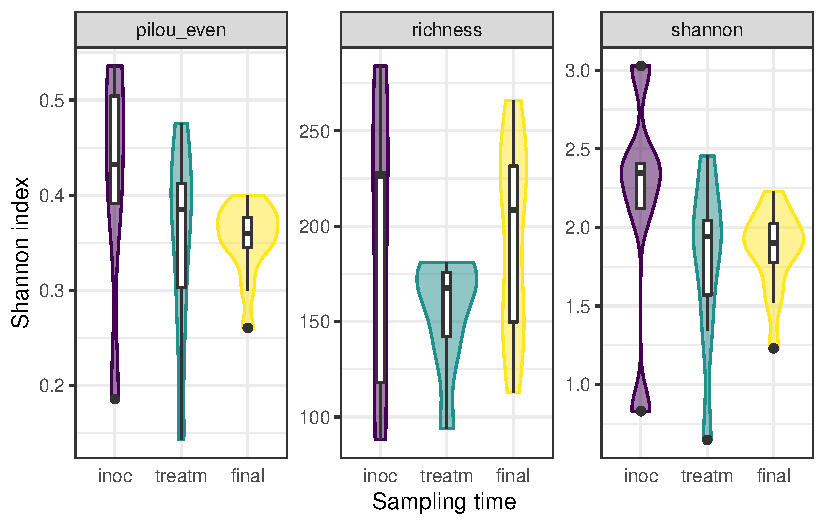
\includegraphics{figures/fig-shannon-byoc-1.pdf}

}

\caption{\label{fig-shannon-byoc}Plot of Shannon Index across experiment
samples grouped by sampling time.}

\end{figure}

After contamination removal, samples consisted of 88 and 284 with a mean
of 181.59. We used the Shannon Index to assess the species diversity and
richness in our samples over the course of the experiment. Samples were
grouped into sampling categories due to low sample sizes on sampling
days (inoc = days 0, 3, 5; treatm = days 7, 9, 12, 15; final = day 24).
There was a slight decrease in mean alpha diversity between inoculation
(M = 2.1458561, sd = 0.8082455) and treatment and final samples (M =
1.7752494, 0.5678242; 1.8578819, 0.260961), as well as a decrease in
variance within samples types (Figure~\ref{fig-shannon-byoc}). Based on
the similarity of distribution between Pielou's Species Evenness and the
Shannon index, the main driver of differences is likely the species
richness (Supp. Mat).

\hypertarget{medium-and-model-calculus-samples-are-distinct-from-the-inoculate}{%
\subsubsection{Medium and model calculus samples are distinct from the
inoculate}\label{medium-and-model-calculus-samples-are-distinct-from-the-inoculate}}

\begin{figure}

{\centering 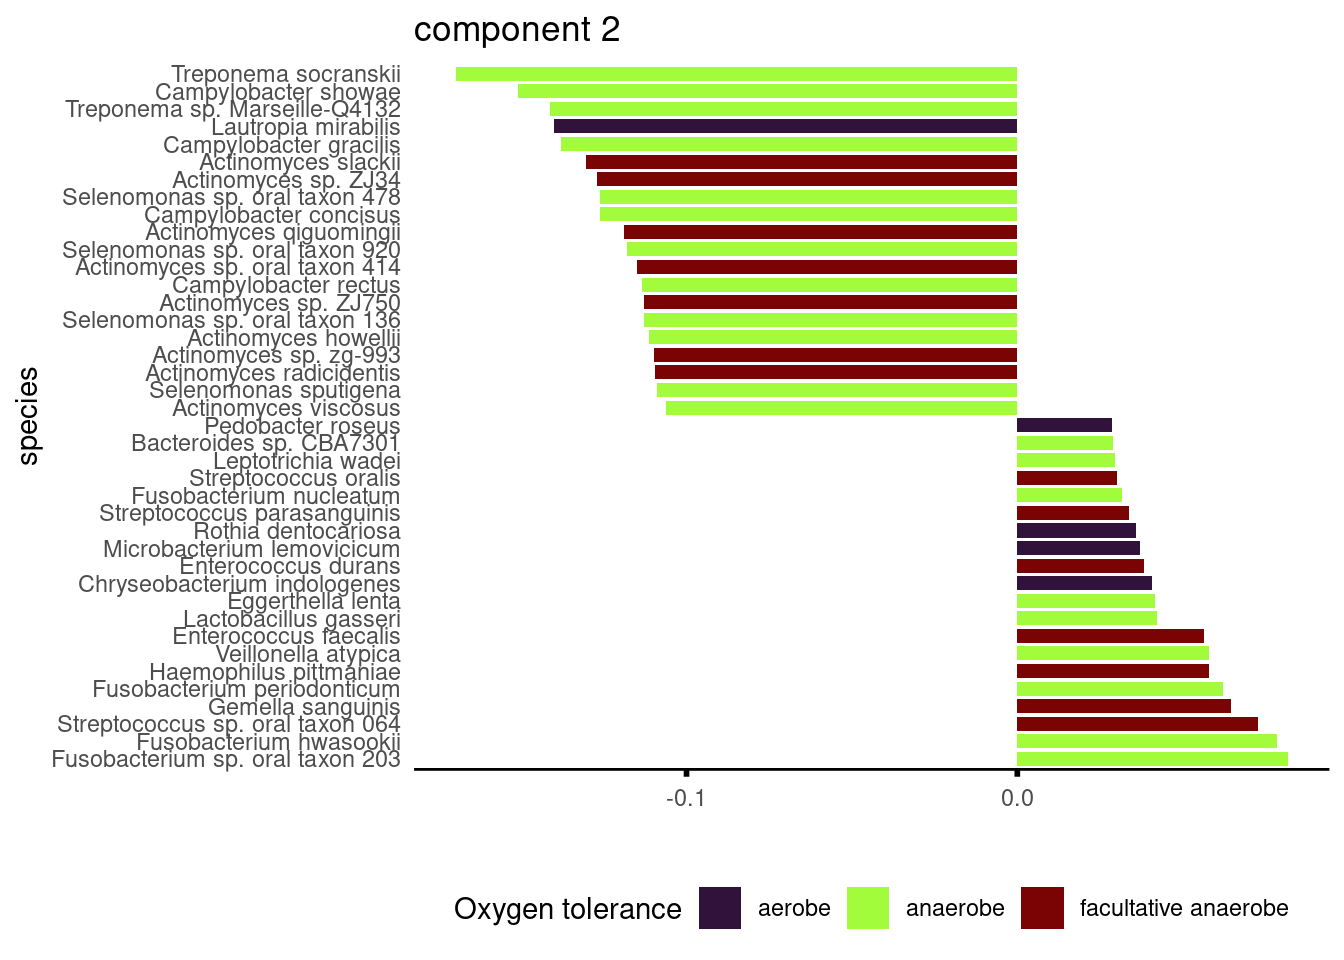
\includegraphics{figures/spca-byoc-plot-1.pdf}

}

\caption{sPCA on species-level counts from experiment samples only.}

\end{figure}

\begin{figure}

{\centering 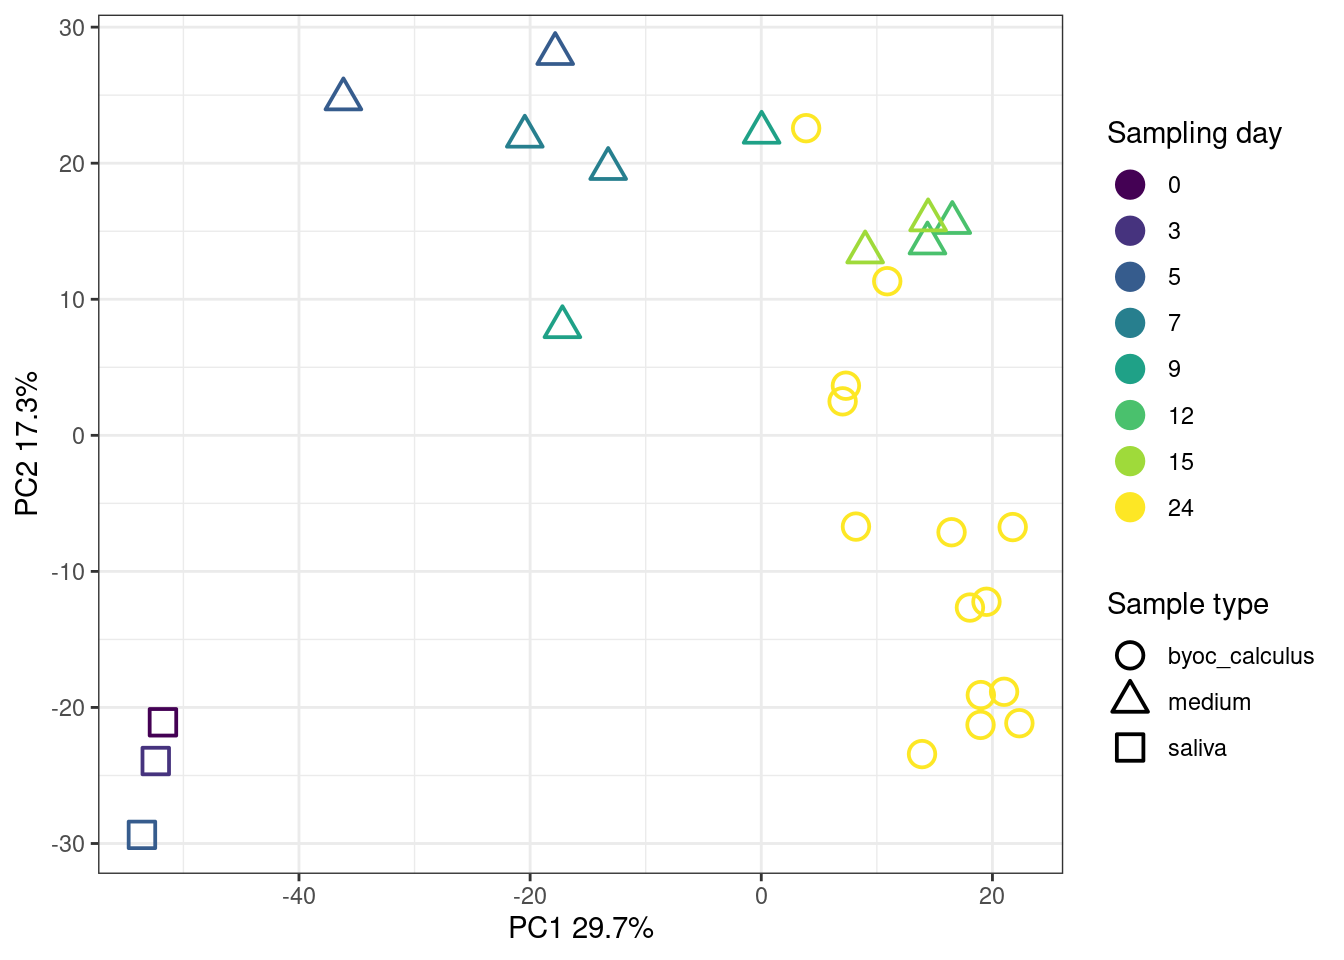
\includegraphics{figures/spca-byoc-plot-2.pdf}

}

\caption{sPCA on species-level counts from experiment samples only.}

\end{figure}

\begin{figure}

{\centering 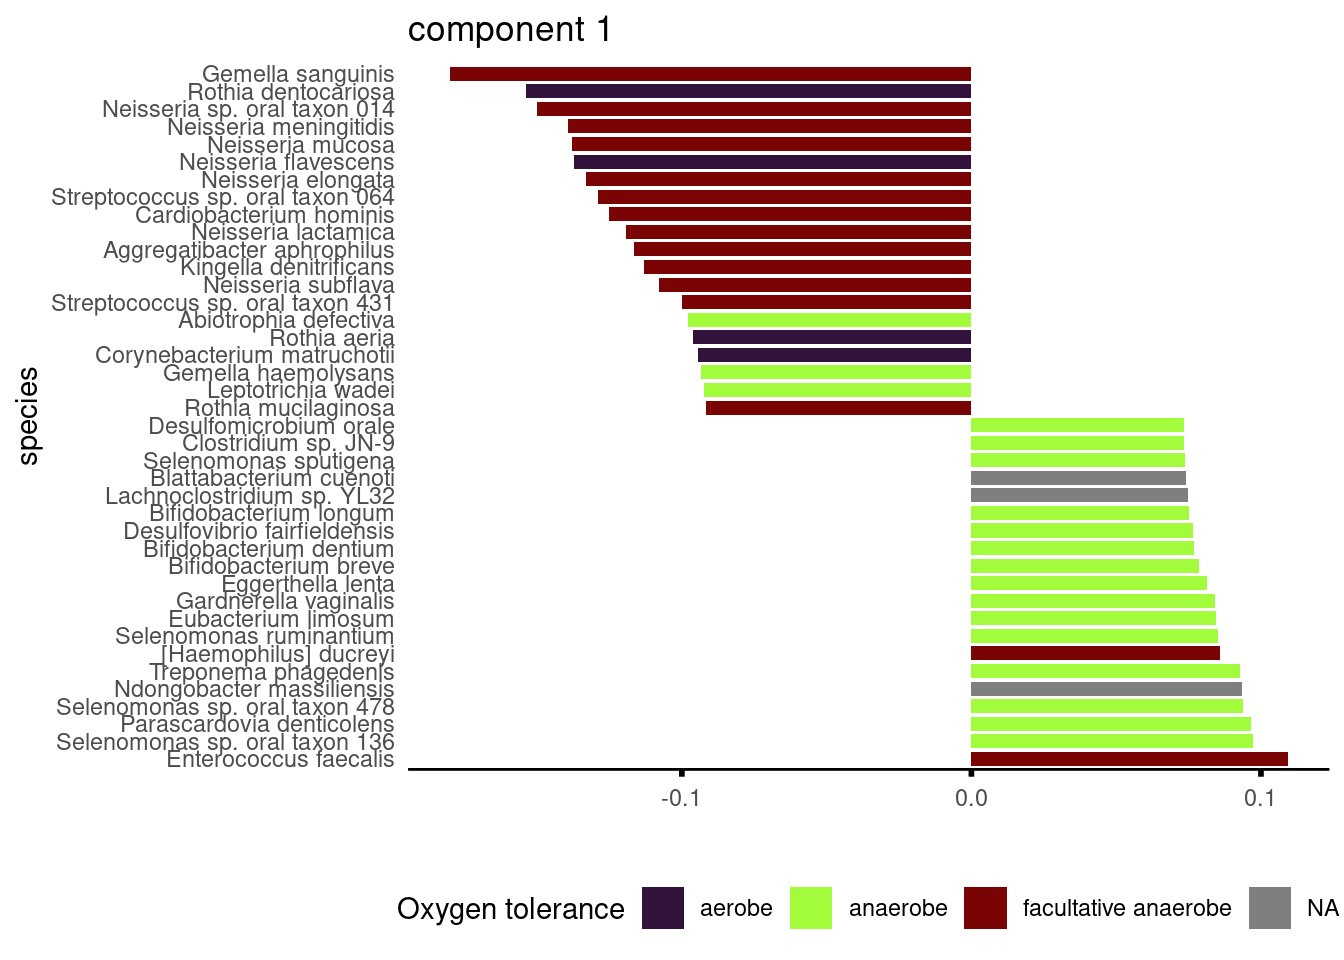
\includegraphics{figures/spca-byoc-plot-3.pdf}

}

\caption{sPCA on species-level counts from experiment samples only.}

\end{figure}

The species profiles of the saliva inoculate used in our experiment were
distinct from both medium and model calculus samples. Most of the
separation is on PC1 of the sPCA, with minimal separation on PC2. Most
of the model calculus samples also cluster separately from the medium
samples on PC2, but maintaining some overlap with more mature medium
samples. The largest negative loadings on PC1, separating inoculate from
other samples, are an abundance of aerobes and facultative anaerobes in
the inoculate, especially \emph{Rothia} and \emph{Neisseria} spp.
Conversely, positive loadings consist mainly of anaerobes, especially
\emph{Selenomonas} spp.

\begin{figure}

{\centering 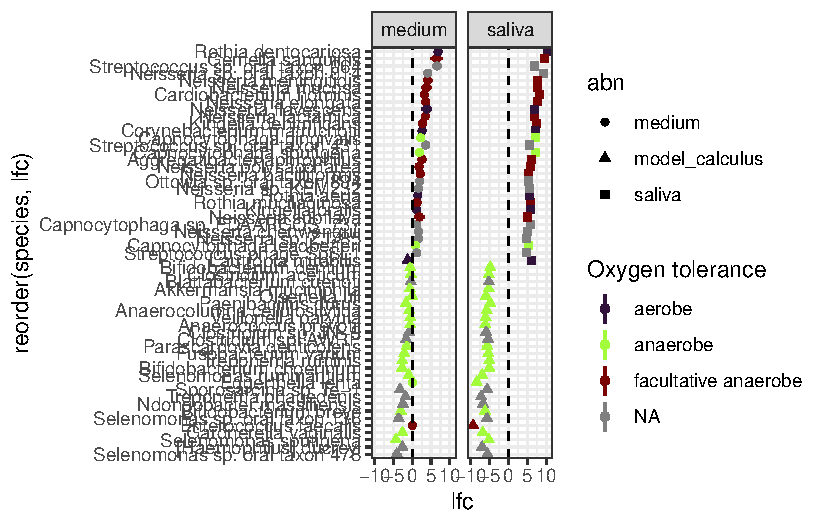
\includegraphics{figures/fig-diffabund-byoc-1.pdf}

}

\caption{\label{fig-diffabund-byoc}Log-fold changes between sample
types. Circles are species enriched in the model calculus, squares are
enriched in saliva, and triangles in medium. Lines are standard error.
Plot shows the top 20 absolute log-fold changes between model calculus
and saliva.}

\end{figure}

Species enriched in saliva compared to model calculus are largely
aerobic or facultative anaerobic, while species enriched in model
calculus compared to saliva are mainly anaerobes. Compared to saliva,
species differences between medium and model calculus are less
pronounced Figure~\ref{fig-diffabund-byoc}.

\hypertarget{lower-diversity-in-artificial-samples-than-oral-references}{%
\subsubsection{Lower diversity in artificial samples than oral
references}\label{lower-diversity-in-artificial-samples-than-oral-references}}

\begin{figure}

{\centering 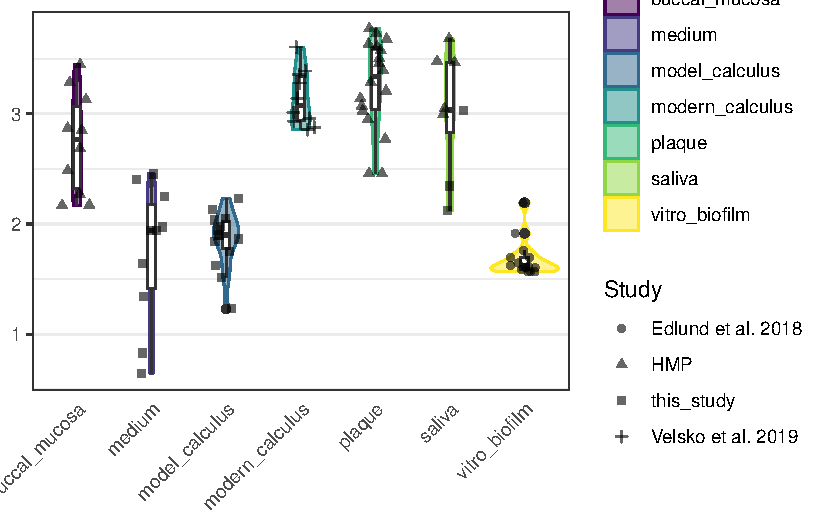
\includegraphics{figures/fig-shannon-compar-1.pdf}

}

\caption{\label{fig-shannon-compar}\textbf{?(caption)}}

\end{figure}

Again, the Shannon Index was used to evaluate alpha diversity, this time
across model samples and oral reference samples. Model samples (M =
1.86, M = 1.74, M = 1.69) were consistently lower than oral reference
samples (M = 2.74, M = 3.14, M = 3.02, M = 3.53, M = 3.04) in species
richness and diversity. The Pielou Species Evenness has a similar
distribution, although the comparative biofilm samples have a higher
mean than biofilm samples from this study (Supp. Mat.).

\hypertarget{model-calculus-is-distinct-from-dental-calculus-and-other-oral-samples}{%
\subsubsection{Model calculus is distinct from dental calculus and other
oral
samples}\label{model-calculus-is-distinct-from-dental-calculus-and-other-oral-samples}}

\begin{figure}

{\centering 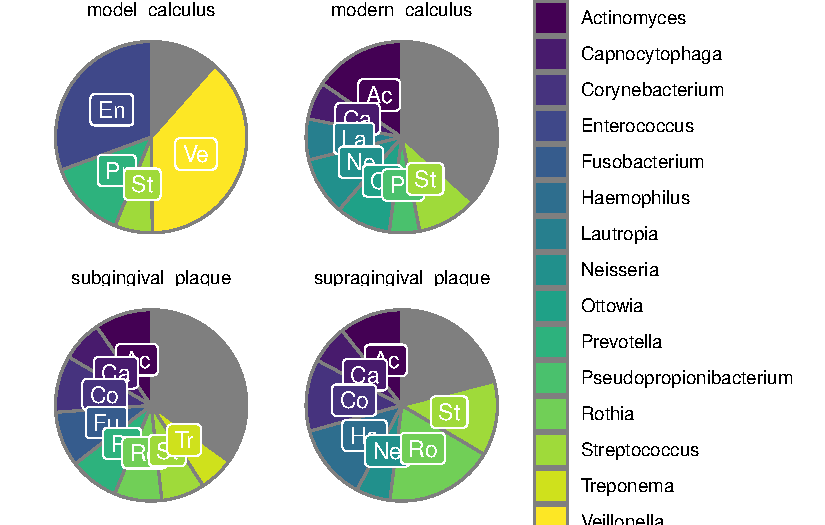
\includegraphics{figures/fig-genus-env-1.pdf}

}

\caption{\label{fig-genus-env}Core microbiome of the different types of
samples represented as mean relative abundances at the genus level. NA =
other genera.}

\end{figure}

The main overlap between the model calculus and oral comparative samples
are the high relative abundance of \emph{Streptococcus}. Model calculus
consists mostly of \emph{Enterococcus} and \emph{Veillonella} spp.,
while oral comparative samples are more diverse (consistent with the
Shannon Index).

\begin{figure}

{\centering 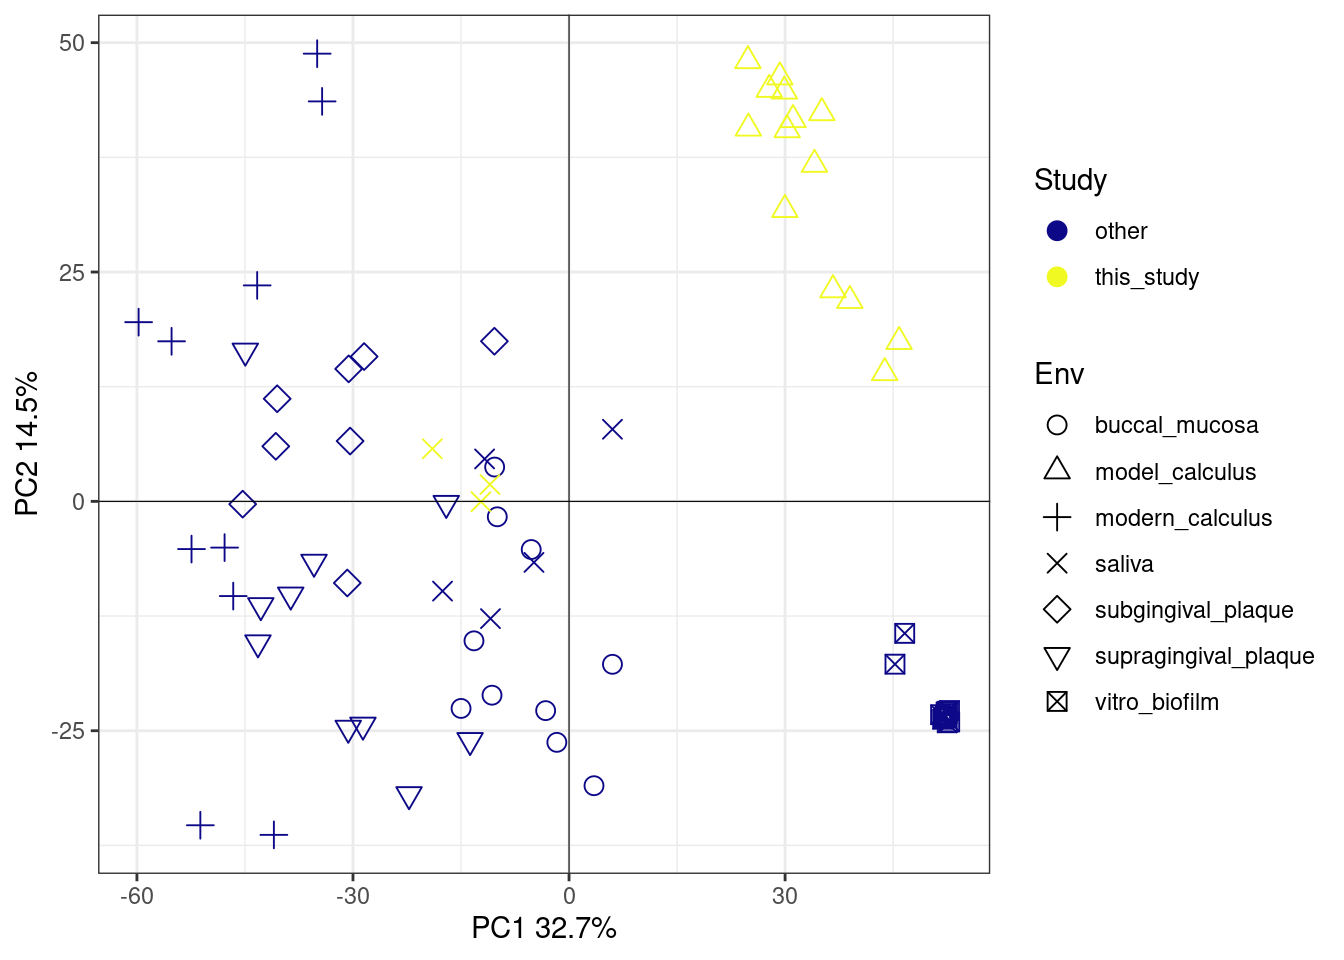
\includegraphics{figures/unnamed-chunk-14-1.pdf}

}

\end{figure}

\begin{figure}

{\centering 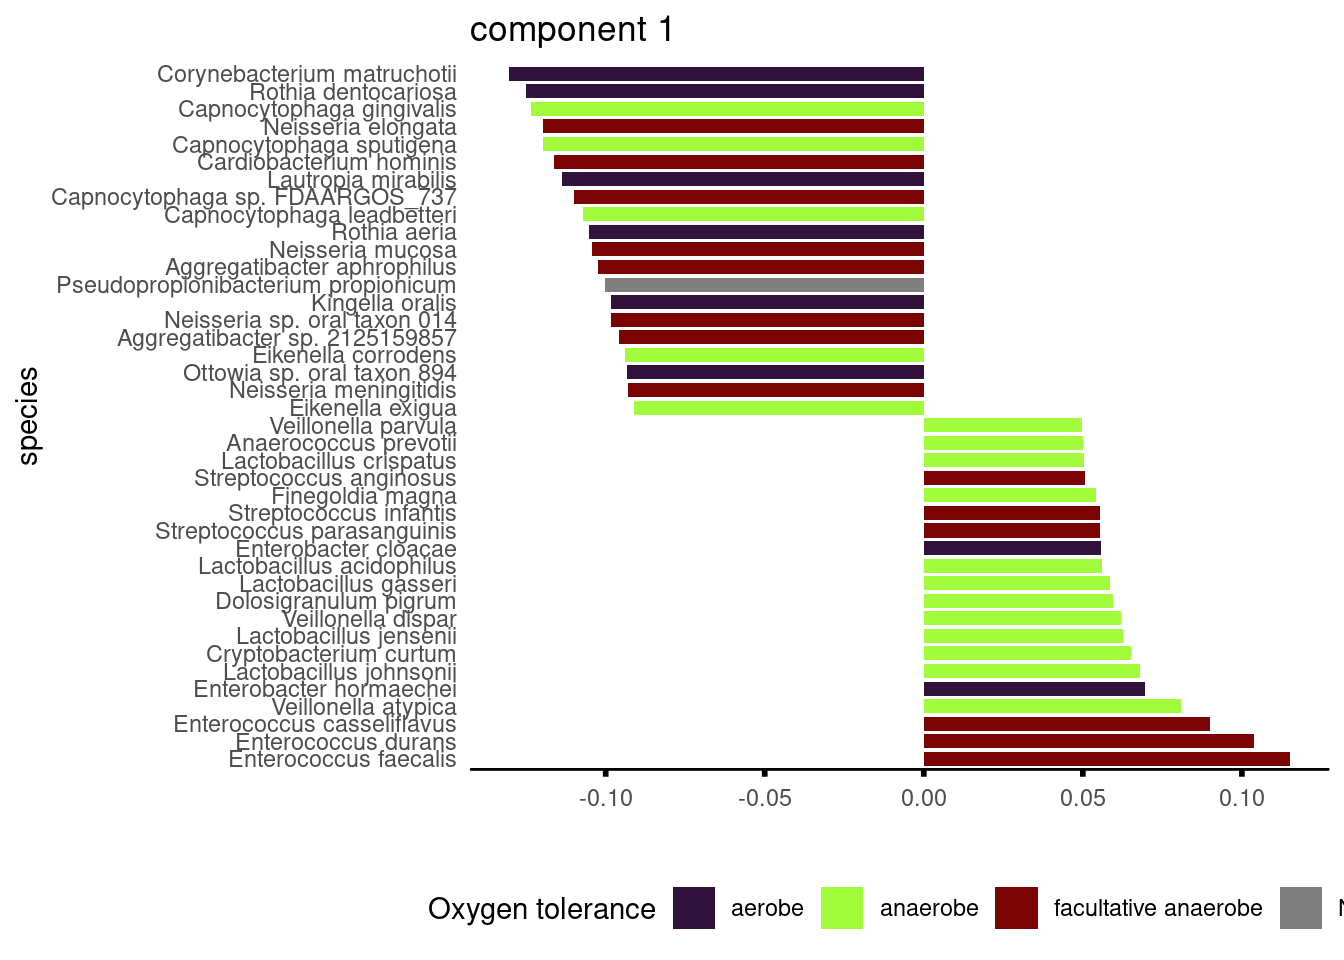
\includegraphics{figures/unnamed-chunk-14-2.pdf}

}

\end{figure}

\begin{figure}

{\centering 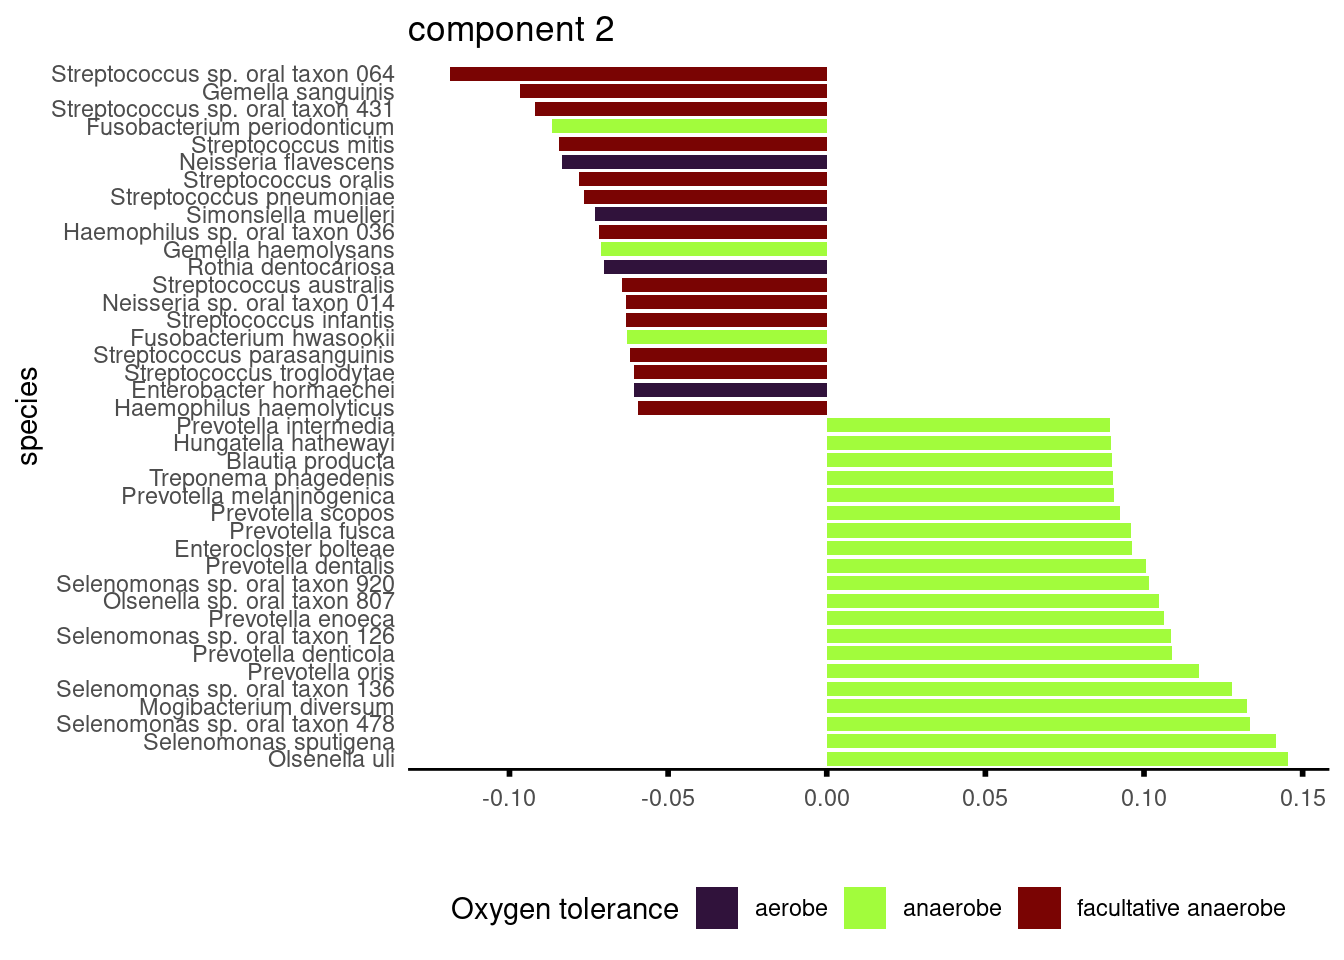
\includegraphics{figures/unnamed-chunk-14-3.pdf}

}

\end{figure}

Model calculus samples are distinct from both the oral reference samples
and the biofilm model reference samples. They are separated from oral
reference samples mainly on PC1, and from biofilm model reference
samples (and, to some extent, oral samples) on PC2. The highest negative
contributions are a mix of all types of aerotolerance, while the
positive contributions are mostly (facultative) anaerobes, with
\emph{Enterococcus} spp. as the top three positive contributors to PC1.
Top negative contributors are \emph{Capnocytophaga} spp as well as the
aerobes \emph{Corynebacterium matruchotii} and \emph{Rothia
dentocariosa}. The top positive contributors to PC2 are all anaerobes,
mainly from the genus \emph{Selenomonas}. Top negative contributors to
PC2 are a mix of aerotolerances, with many \emph{Streptococcus} spp.

\begin{figure}

{\centering 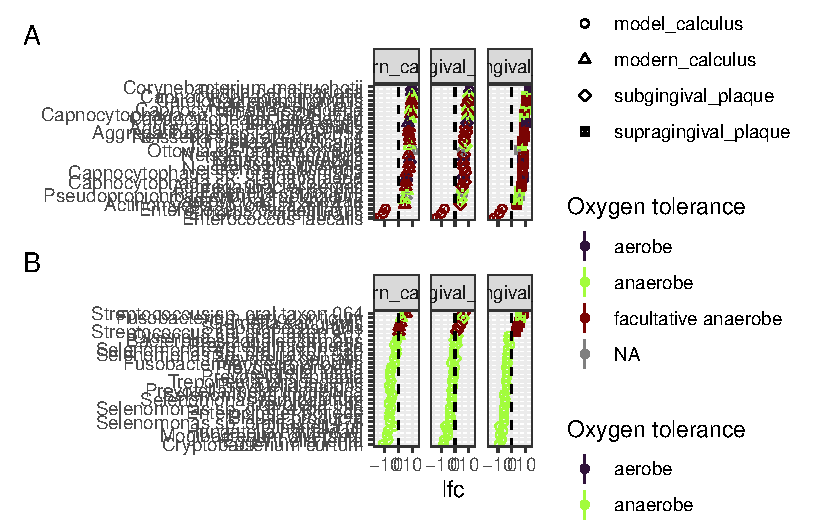
\includegraphics{figures/fig-diffabund-comp2-1.pdf}

}

\caption{\label{fig-diffabund-comp2}Log-fold changes between sample
types. Circles are species enriched in the model calculus, triangles in
modern calculus, diamonds are enriched in subgingival plaque, and
squares in supragingival plaque. Plot shows the top 30 loadings
(absolute value) in PC1 (A) and PC2 (B) between model calculus and other
sample types, ordered by decreasing log-fold change. Bars represent
standard error.}

\end{figure}

Based on the differential abundance analysis on the top loadings from
PC1, the main differences between model calculus and oral reference
samples, are that the oral reference samples are enriched with species
with a diverse oxygen tolerance from a wide range of genera, while the
model calculus is enriched with \emph{Enterococcus} spp. The largest
differences occur in \emph{Corynebacterium matruchotii}, \emph{Rothia
dentocariosa}, and \emph{Capnocytophaga gingivalis}
(Figure~\ref{fig-diffabund-comp2}A). This is echoed in the differential
abundance analysis on top loadings from PC2, where most of the species
are enriched in model calculus, all of which are anaerobes, and the
largest differences occurring in \emph{Cryptobacterium curtum},
\emph{Eggerthella lenta}, and \emph{Mogibacterium diversum}
(Figure~\ref{fig-diffabund-comp2}B).

\hypertarget{increasing-mineralisation-over-the-course-of-the-experiment}{%
\subsection{Increasing mineralisation over the course of the
experiment}\label{increasing-mineralisation-over-the-course-of-the-experiment}}

\begin{figure}

\begin{minipage}[t]{0.50\linewidth}

{\centering 

\raisebox{-\height}{

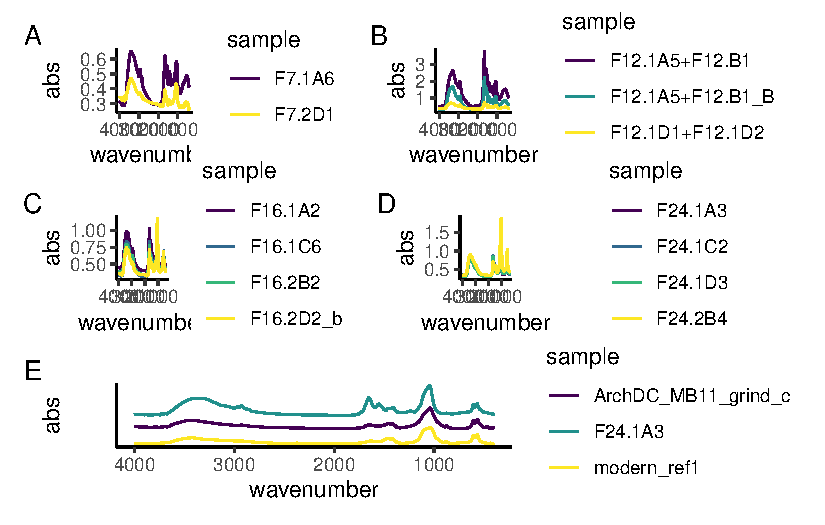
\includegraphics{figures/fig-experiment-spectra-1.pdf}

}

}

\subcaption{\label{fig-experiment-spectra-1}Spectra from day 7 samples.}
\end{minipage}%
%
\begin{minipage}[t]{0.50\linewidth}

{\centering 

\raisebox{-\height}{

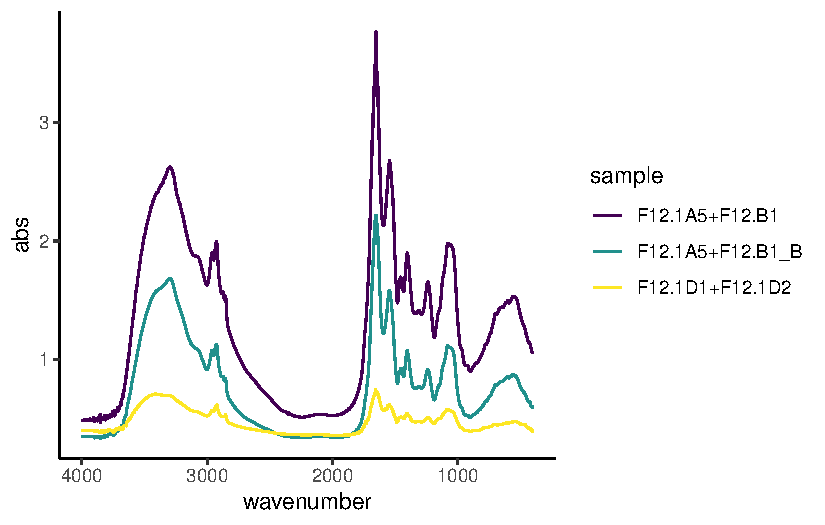
\includegraphics{figures/fig-experiment-spectra-2.pdf}

}

}

\subcaption{\label{fig-experiment-spectra-2}Spectra from day 12
samples.}
\end{minipage}%
\newline
\begin{minipage}[t]{0.50\linewidth}

{\centering 

\raisebox{-\height}{

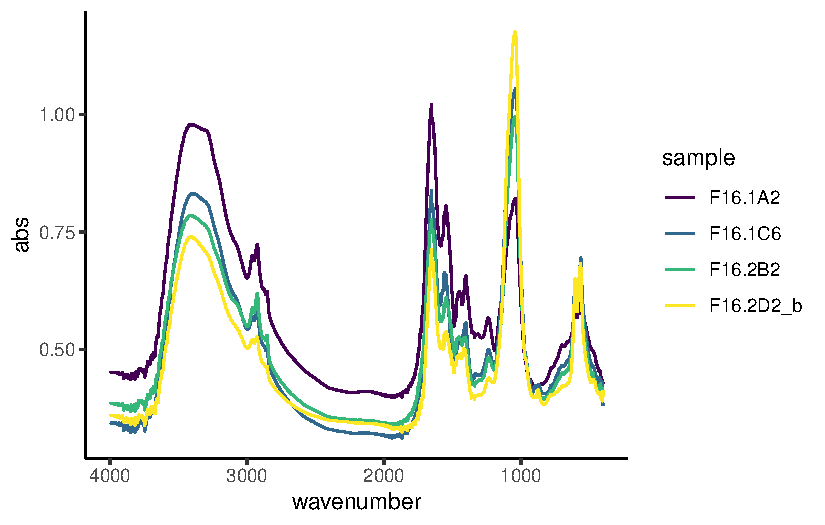
\includegraphics{figures/fig-experiment-spectra-3.pdf}

}

}

\subcaption{\label{fig-experiment-spectra-3}Spectra from day 16
samples.}
\end{minipage}%
%
\begin{minipage}[t]{0.50\linewidth}

{\centering 

\raisebox{-\height}{

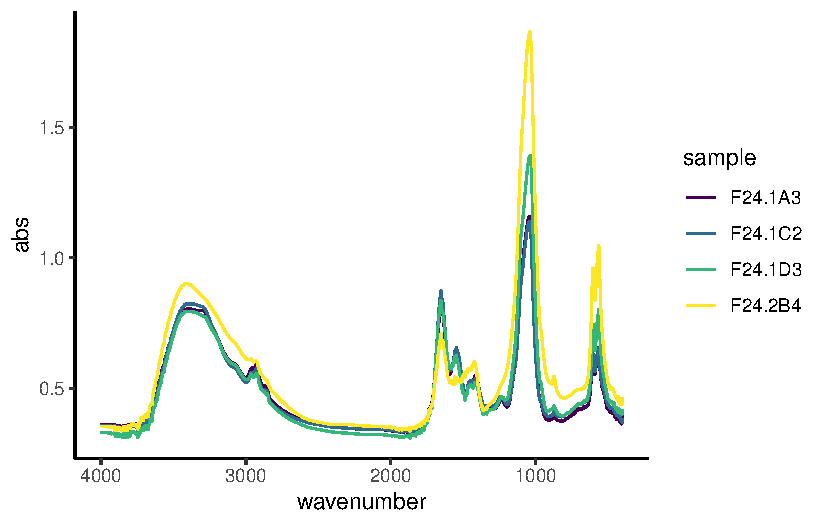
\includegraphics{figures/fig-experiment-spectra-4.pdf}

}

}

\subcaption{\label{fig-experiment-spectra-4}Spectra from day 24 samples
(final product).}
\end{minipage}%

\caption{\label{fig-experiment-spectra}Select spectra from all
experiment sampling days.}

\end{figure}

Day 7 spectra have large O--H and amide A absorbance bands in stretching
mode around 3400 cm\(^{-1}\), as well as three marked
CH\textsubscript{3} and CH\(_2\) stretching vibrations at 2960, 2920,
and 2850 cm\(^{-1}\). There is a clear amide I peak at 1650 and a less
pronounced amide II peak at 1545 cm\(^{-1}\). In the `fingerprint'
region, C--O\(_3^{2-}\) at 1450 and 1400 absorbance bands corresponding
to the v\textsubscript{3} asymmetric stretching vibrations,
P--O\textsubscript{4} absorbance band corresponding to the
v\textsubscript{3} asymmetric stretching vibrations at 1080 cm\(^{-1}\),
and minor phosphate absorption bands around 500 cm\(^{-1}\) in sample
F7.1A6, but absent in sample F7.2D1. The absorption bands at 1080
cm\(^{-1}\), and 1040-1047 cm\(^{-1}\) and minor bending absorption
bands of the phosphate doublet around 605 cm\(^{-1}\) and 560
cm\(^{-1}\) in sample F7.2D1, but absent in sample F7.1A6. The relative
absorbance of O--H and Amide I and II bands are higher than the
phosphate bands, representing a relatively higher content of lipids and
proteins than inorganic content. Large variation between spectra.

Day 12, amide I and II continue to be the dominant peaks, and a higher
ratio of both amide and O--H to PO\textsubscript{4} v\textsubscript{3}
absorbance bands. Three marked CH\textsubscript{3} and CH\(_2\)
stretching vibrations at 2960, 2920, and 2850 cm\(^{-1}\). Reduced
variation between two of the three spectra.

Day 16, the ratio of O--H and amides to PO\textsubscript{4} has shifted,
with the main peak shifting to the PO\textsubscript{4}
v\textsubscript{3} absorbance band at 1040 (except in sample F16.1A2). A
well-defined PO\textsubscript{4} doublet at 600 and 560 is present.
Small CO\(_3^{2-}\) asymmetric stretching at 1450 cm\(^{-1}\) and 1415
cm\(^{-1}\), and stretching vibrations at 875-870 cm\(^{-1}\). Decreased
variability between the spectra, with most spectra exhibiting a higher
phosphate-to-protein/lipid ratio.

Day 24, large O--H and amide A absorbance bands in stretching mode
around 3400 cm\(^{-1}\), as well as three minor CH\textsubscript{3} and
CH\(_2\) stretching vibrations at 2960, 2920, and 2850 cm\(^{-1}\). Main
peak of spectra is PO\textsubscript{4} v\textsubscript{3} at 1040
cm\(^{-1}\), well-defined PO\textsubscript{4} doublet at 600-550
cm\(^{-1}\). Amide I band, with small amide II and III bands. Carbonate
peaks also present. Very little variation between all of the spectra.

\begin{figure}

{\centering 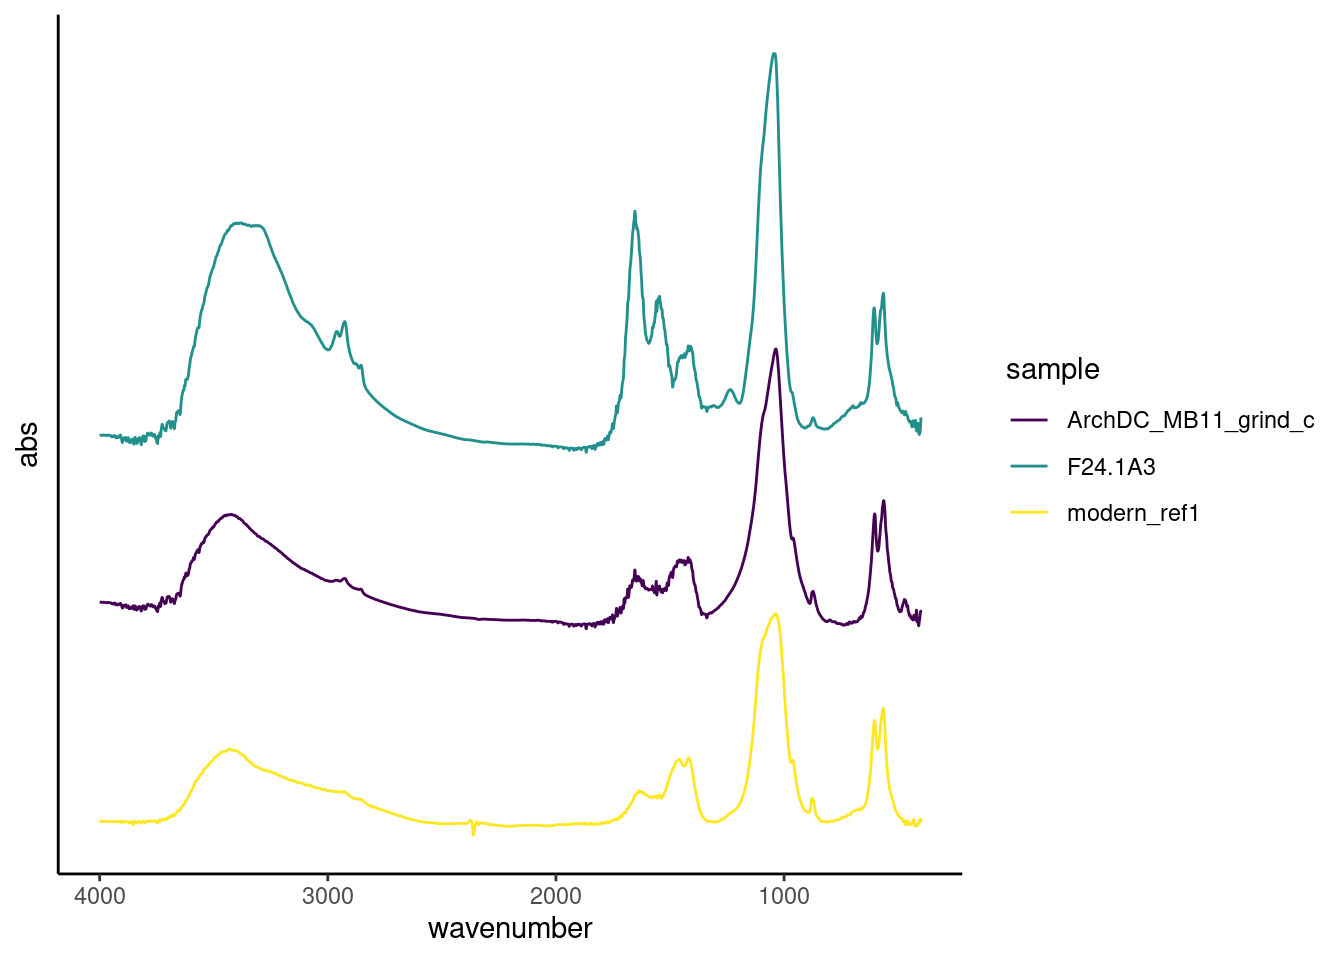
\includegraphics{figures/compare-calc-spectra-1.pdf}

}

\caption{Spectra from archaeological calculus, modern reference
calculus, and artificial calculus are compared. Absorbance was shifted
to allow comparison of the three spectra, so the absorbance should be
interpreted as relative, not absolute.}

\end{figure}

The archaeological and modern reference spectra are largely
indistinguishable and consist of an O--H absorbance band (3400
cm\(^{-1}\)), CH\textsubscript{3} bands (3000--2900 cm\(^{-1}\)),
carbonate (1420, 1458-1450, 875-870 cm\(^{-1}\)), amide I band (1650
cm\(^{-1}\)), and phosphates (1040, 604, 566 cm\(^{-1}\)). The model
calculus samples from the end of the experiment are similar to both
reference samples. The main difference is a lower organic component in
reference samples seen as a reduced amide I peak at around 1637 compared
to the carbonate peak at around 1420, and an absence of amide II and
III. Also a reduction in CH\textsubscript{3} bands at 3000-2900
cm\(^{-1}\).

\hypertarget{similar-crystallinity-and-order-compared-to-reference-calculus}{%
\subsubsection{Similar crystallinity and order compared to reference
calculus}\label{similar-crystallinity-and-order-compared-to-reference-calculus}}

\begin{figure}

{\centering 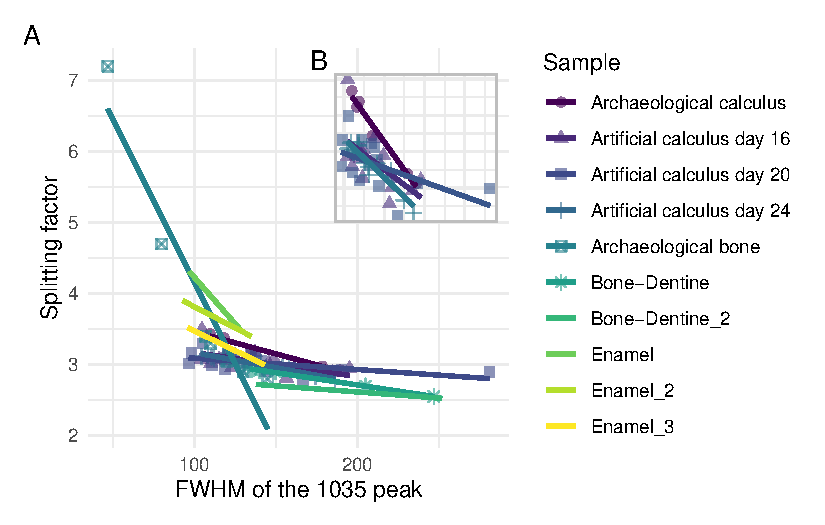
\includegraphics{figures/fig-grind-curve-1.pdf}

}

\caption{\label{fig-grind-curve}(A) Grinding curves of multiple
materials; and (B) calculus-only materials, including biofilm samples
from three days, and an archaeological calclulus sample.}

\end{figure}

Samples were compared to the results of Asscher, Regev, et al. (2011)
and Asscher, Weiner, et al. (2011), and the slopes of the trend lines
for our model calculus are similar to those of fresh bone and dentin. No
appreciable differences between days 16, 20, and 24. The archaeological
dental calculus does show a slightly increased slope compared to model
calculus from the three sampling days used in the grind curve.

\hypertarget{discussion}{%
\section{Discussion}\label{discussion}}

In this study we present a {[}long-term{]} oral biofilm model with
mineralisation to produce artificial dental calculus. Our proposed use
of the model is to address a variety of research questions related to
dietary information extracted from dental calculus, in both modern and
ancient samples. For that to be feasible, the model needs to act as a
viable proxy to dental calculus grown under natural conditions, i.e., in
the human mouth. It needs, as much as possible, to mimic the diversity
and complexity of the natural oral microbiome, while also offering
control over factors such as dietary input, growth conditions, and
replicability within and between experiments. Here, we assessed the
viability of our model as a proxy for dental calculus using metagenomic
classification and FTIR analysis to explore the bacterial and mineral
composition, and compare with oral reference samples.

\hypertarget{microbiome}{%
\subsection{Microbiome}\label{microbiome}}

There is a loss of diversity from donated saliva to model calculus, and
when compared to oral reference samples, which is a common limitation in
biofilm models (Bjarnsholt et al., 2013; Edlund et al., 2013). The
donated saliva for the experiment had a lower diversity than the
reference saliva samples, and may have contributed to a lower diversity
in experiment samples. Consequently, there is also a lower diversity and
richness when compared to other modern oral reference samples, including
oral mucosa, saliva, plaque, and calculus. Model calculus samples
primarily consist of species within the genera \emph{Veillonella} and
\emph{Enterococcus}, with more limited contributions from
\emph{Streptococcus} and \emph{Prevotella}. The core microbiomes of oral
reference samples have similar levels of streptococci, but a much more
even distribution of species from \emph{Actinomyces},
\emph{Capnocytophaga}, \emph{Fusobacterium}, and more.

Medium samples from early in the experiment have similar species
profiles to the donated saliva, but gradually diverge over the course of
the experiment, as seen in the increasing separation of samples on PC1
in Figure. This may be caused by the growth conditions provided by the
experimental setup, which may not sufficiently mimic the oral
environment, allowing different oral species to thrive that do not
normally thrive in the natural oral environment. Especially
\emph{Enterococcus} spp. seemed to thrive later in the experiment, at
the expense of more fastidious species like \emph{Capnocytophaga} and
\emph{Neisseria} spp., which require an atmosphere with at least 5\%
carbon dioxide to thrive, so the model may have a low carbon dioxide
atmosphere (Tønjum \& van Putten, 2017). Early colonisers, including the
aforementioned \emph{Capnocytophaga} and \emph{Neisseria} spp., as well
as \emph{Actinomyces}, were dominant in oral reference samples and
deficient in model calculus samples, as well as the comparative \emph{in
vitro} model. Not only is there a decreased species diversity between
model and reference samples, but also a loss of diversity in
aerotolerance. Of the dominant species in the model, most are either
anaerobes or facultative anaerobes, predominantly Gram-negative
\emph{Veillonella} and \emph{Prevotella}, and Gram-positive
\emph{Enterococcus}. Species within predominantly aerobic genera, such
as \emph{Neisseria}, \emph{Rothia}, and \emph{Ottowia}, are deficient in
the model compared to the donated saliva and other oral samples,
suggesting a shift from a largely aerotolerant profile to an anaerobic
profile during the experiment. While our model is not set up as an
anaerobic system, the anaerobes seem to have outcompeted aerobes and, to
some extent, facultative anaerobes. This is likely a result of
communities of bacteria within the biofilm creating favourable
microenvironments facilitated by the protective properties of the
biofilm matrix (Edlund et al., 2018; Flemming et al., 2016).
\emph{Capnocytophaga} and \emph{Actinomyces} spp. are predominantly
(facultative) anaerobes, so their deficiency must be attributed to
different reasons. The highest log-fold changes between model calculus
and other samples were seen in \emph{E. faecalis}, \emph{E. durans}, and
\emph{E. casseliflavus}, and contributed most to the unique clustering
of model calculus on PC1. \emph{E. faecalis} was also abundant in the
comparative \emph{in vitro} biofilm study. \emph{Enterococcus} spp.
out-competing other species may be a problem in model biofilm studies,
but more comparative studies are needed to confirm (and there are
limited WGS studies to use as a comparison).

Model calculus and the modern reference calculus clustered separately in
the sPCA analysis. This may be due to human variation, as there can be
large differences in the oral microbiome of two individuals, and modern
reference samples were taken from the same geographical origin (as was
the donor saliva for the model, which was taken from a different
geographical origin). One of the main drivers of differences in species
profiles has been previously shown to be individual variation, even more
so than pathological condition (Velsko et al., 2022). Whether or not
distinct microbial profiles will affect the retention of dietary
incorporation remains to be seen, and likely depends on the role
bacteria play in the incorporation and retention of dietary compounds
and microremains within a biofilm. Samples within the experiment were
quite consistent allowing this to be explored further.

Species related to caries, such as \emph{Steptococcus mutans} and
members of the \emph{Lactobacillus} genus, were deficient in both model
calculus samples and oral reference samples. Both are integral in
creating an acidic environment that favours demineralisation and
inhibits mineralisation, so there absence is expected in a calculus
model (Edlund et al., 2013; Velsko et al., 2019). The abundance of
\emph{Veillonella} and \emph{Prevotella} spp. could suggest a pathogenic
potential within the model biofilm, as these are commonly reported as
opportunistic or accessory pathogens in periodontal disease (Tett et
al., 2021; Zhou et al., 2021).

\hypertarget{mineralisation}{%
\subsection{Mineralisation}\label{mineralisation}}

FTIR analysis allowed us to address the mineralisation process of the
model. The results showed an increasing mineral composition over the
course of the experiment as the model biofilm matured. Samples taken
early in the experiment, on day 7 and 12, had a high lipid and protein
content consistent with the presence of microbial DNA and RNA within a
matrix of extracellular polysaccharides (Jain et al., 2013). The high
water content, indicated by the O--H stretch, is also consistent with a
biofilm, which is around 90\% water (Berger et al., 2018). As the
samples mature over the course of the experiment, the ratio of proteins
and lipids to phosphates shift from predominance of organic content to
inorganic content in the form of carbonated hydroxyapatite.

The artificial samples from day 24 are consistent with spectra of
carbonated hydroxyapatite and resemble both the modern reference samples
and the archaeological sample in mineral composition and crystallinity.
The steeper slope in the grind curve plots of the archaeological sample
may suggest that the crystals in archaeological samples are larger than
in the model calculus Figure~\ref{fig-grind-curve}. A possible
explanation is that the inorganic crystals within archaeological
calculus have had more time to expand into the space left by degraded
organic matter (Weiner, 2010b). It may also have been an unusually
crystallised sample; as we only analysed a single archaeological sample,
and more modern and archaeological samples are needed to see if the high
level of crystallinity is consistent in archaeological calculus, and if
the level of crystallinity of the model calulus is more comparable to
modern reference samples. The grinding curves for days 16, 20, and 24
were very similar, suggesting that the CPMU solution, which is
introduced on day 16 to promote mineralisation, may not have much of an
effect.

Although there were differences in species profiles between modern and
model calculus, the mineral composition of the end results were similar,
reinforcing the idea that, under the right circumstances, most bacteria
will mineralise (Moorer et al., 1993). Even occurring without one of the
most well-known biomineraliser, \emph{Corynebacterium matruchotii},
which was deficient in model, and was the strongest discriminator of
oral samples from model samples. It may also suggest that, while
bacteria are integral in the formation of dental calculus, and
inevitably serve as part of the structure that dental calculus is built
upon (Rohanizadeh \& LeGeros, 2005), the species composition of the
biofilm communities may be less important. And that mineralisation may
largely be a chemical process (catalysed by biological factors) (Omelon
et al., 2013).

\hypertarget{replicability}{%
\subsection{Replicability}\label{replicability}}

The model calculus displayed similar species diversity and richness
indices across all samples, indicating a high level of replicability
between samples in the experimental run, despite larger variation
between medium samples. Both sPCA analyses conducted with experiment
only samples and with oral reference samples also cluster model calculus
closely together. It remains to be seen whether the replicability within
the experiment also scales up to between-experiment replicability. The
variation in mineral composition was initially high in early model
biofilm samples from days 7 and 12, but starting day 16 the variation
decreased, and continued to decrease until day 24. The model calculus
samples from day 24 were largely similar in composition as observed in
the FTIR spectra. The use of a simple multiwell plate setup allows us to
{[}submit{]} many samples to the same conditions which promotes
replicability between samples. While the experimental conditions,
including the dietary input, are kept constant, and the mineral and
bacterial profiles are similar between samples, there is still a
relatively large variation in starch retention in the model calculus
(Bartholdy \& Henry, 2022).

There are many biofilm models to choose from, so developing a new
protocol may seem counter-productive; however, few are developed for
long-term growth and even fewer for mineralisation. One of the
exceptions involves a complex setup that is likely unfeasible to most
archaeological research (Sissons et al., 1991). Our model uses a
simplified high-throughput setup more commonly seen in shorter-term
biofilm models that mainly focus on dental plaque (Exterkate et al.,
2010; Tian et al., 2010). As shown in a previous study, calculus and
plaque have distinct microbial profiles (Velsko et al., 2019), so their
applicability to explore archaeological questions on dental calculus are
limited. Clinical studies are also largely focused on short-term effects
of anti-microbial treatments and inhibition of biofilm formation, while
archaeologists are more interested in questions related to \ldots{}
Questions, we believe, can to some extent be answered using an oral
biofilm model. Our previous work has shown that, like dental calculus,
the model calculus is able to trap and retain dietary starches,
admittedly with some variability between samples (Bartholdy \& Henry,
2022).

\hypertarget{limitations}{%
\subsection{Limitations}\label{limitations}}

A well-known limitation of biofilm models is the difficulty in capturing
the diversity and complexity of the natural oral biome. Diversity and
complexity may be represented as interspecies communities and complex
metabolic dependencies between organisms within the communitues, or as
an environmental complexity determined by nutrient availability, host
immune-responses to biofilms, and fluctuating microenvironments across
the biofilm in response to these factors (Bjarnsholt et al., 2013;
Edlund et al., 2018). Our single-donor approach may have affected
diversity of model. The donated saliva had a lower mean alpha-diversity
than other saliva samples. Although benefit of single donor means
maintaining the integrity of the original bacterial community. There are
benefits and trade-offs for both pooled and single-donor saliva (Edlund
et al., 2013).

Research relating to \(alpha\)-amylase activity and its effect on the
oral biome (whether dietary or otherwise) will require addition of
amylase to the model during the experiment, as it is not present
naturally in our current setup (as shown in Bartholdy \& Henry (2022)).
Our model has no renewable source for \(alpha\)-amylase once the
inoculations have been completed. There are streptococci present in the
model, which are known for their ability to bind amylase (Nikitkova et
al., 2013); however, it is unclear whether the correct strains are
present in our model, and if they are, why they are not binding
\(alpha\)-amylase provided by the saliva inoculate. This could be due to
the frequency of medium replacement potentially clearing out all of the
unbound amylase every time medium is replaced. Our current model does
not contain serum, which may be contributing to the deficiency of
slow-growing fastidious organisms (Tian et al., 2010).

Biofilms were grown in a standard shaking incubator, rather than a
incubator specific to cell cultures. The lack of complex environmental
control may cause the model to deviate from its natural growth over the
24 days that the experiment is run, due to a lack of precise control
over physiological conditions.

There is also a possibility of contamination in the model. While the
CPMU solution was prepared under sterile conditions, the solution itself
was not autoclaved, and may have been a source of contamination. This is
further \ldots{} by the fact that none of the medium samples taken after
the introduction of CPMU (day 14) made it past authentication in the
metagenomic analysis, and that a large portion of the sources of many
samples were estimated to be from indoor air and surface samples .

Another limitation involves the information on aerotolerance of the
identified species. Species-level aerotolerance was collected from
BacDive and, at the time of writing, 55.9\% species were missing
aerotolerance values. This was mitigated by aggregating genus-level
tolerances to missing species, and may have some errors (although
unlikely to make any significant changes).

\hypertarget{future-work}{%
\subsection{Future work}\label{future-work}}

Our goals for additional validation measures involve functional profiles
of bacterial, to see if metabolic behaviour of bacteria is consistent
with \emph{in vivo} conditions, and whether this is affected by the
presence/absence of amylase. Further protocol optimisation will also be
necessary to address some of the limitations of our current model. We
may need to reduce the frequency of medium replacement (currently every
three days) to help promote the growth of slower growing organisms and
limit generalists such as enterococci. More infrequent medium
replacement would facilitate slow-growing bacteria in establishing their
metabolic relationships, allowing the byproducts of some species to
become abundant enough for others that depend on these to grow (Marsh,
2005). Finally, if the within-experiment replicability is also present
between experiments. An important question to address is what role
bacteria play in the incorporation and retention of dietary
microremains, and whether differing bacterial profiles affects the
dietary incorporation and retention within the biofilm. Regardless, the
apparent replicability of our current setup is a promising result.

The calculus model we have presented has many potential benefits within
archaeological research. It can be used to test many fundamental
assumptions we have about the process of inclusion and subsequent
extraction of various information about health and diet from
archaeological dental calculus. How our current methods for exploring
diet and health may be biased. How different methods of food processing
in the past may reflect the picture we get from the samples we analyse.
This method can be used for a wide range of methods-testing (e.g.~DNA,
proteomics, etc.) as well as training for various sampling methods, and
testing decontamination protocols, without using up limited supplies of
archaeological resources.

\hypertarget{references}{%
\section*{References}\label{references}}
\addcontentsline{toc}{section}{References}

\hypertarget{refs}{}
\begin{CSLReferences}{1}{0}
\leavevmode\vadjust pre{\hypertarget{ref-adlerSequencingAncient2013}{}}%
Adler, C. J., Dobney, K., Weyrich, L. S., Kaidonis, J., Walker, A. W.,
Haak, W., Bradshaw, C. J., Townsend, G., Soltysiak, A., Alt, K. W.,
Parkhill, J., \& Cooper, A. (2013). Sequencing ancient calcified dental
plaque shows changes in oral microbiota with dietary shifts of the
{Neolithic} and {Industrial} revolutions. \emph{Nature Genetics},
\emph{45}(4), 450--455, 455e1. \url{https://doi.org/10.1038/ng.2536}

\leavevmode\vadjust pre{\hypertarget{ref-asscherAtomicDisorder2011}{}}%
Asscher, Y., Regev, L., Weiner, S., \& Boaretto, E. (2011). Atomic
{Disorder} in {Fossil Tooth} and {Bone Mineral}: {An FTIR Study Using}
the {Grinding Curve Method}. \emph{ArcheoSciences. Revue
d'archéométrie}, \emph{35, 35}, 135--141.
\url{https://doi.org/10.4000/archeosciences.3062}

\leavevmode\vadjust pre{\hypertarget{ref-asscherVariationsAtomic2011}{}}%
Asscher, Y., Weiner, S., \& Boaretto, E. (2011). Variations in {Atomic
Disorder} in {Biogenic Carbonate Hydroxyapatite Using} the {Infrared
Spectrum Grinding Curve Method}. \emph{Advanced Functional Materials},
\emph{21}(17), 3308--3313. \url{https://doi.org/10.1002/adfm.201100266}

\leavevmode\vadjust pre{\hypertarget{ref-bartholdyInvestigatingBiases2022}{}}%
Bartholdy, B. P., \& Henry, A. G. (2022). Investigating {Biases
Associated With Dietary Starch Incorporation} and {Retention With} an
{Oral Biofilm Model}. \emph{Frontiers in Earth Science}, \emph{10}.
\url{https://www.frontiersin.org/articles/10.3389/feart.2022.886512}

\leavevmode\vadjust pre{\hypertarget{ref-bergerOralBiofilms2018}{}}%
Berger, D., Rakhamimova, A., Pollack, A., \& Loewy, Z. (2018). Oral
{Biofilms}: {Development}, {Control}, and {Analysis}.
\emph{High-Throughput}, \emph{7}(3), 24.
\url{https://doi.org/10.3390/ht7030024}

\leavevmode\vadjust pre{\hypertarget{ref-bjarnsholtVivoBiofilm2013}{}}%
Bjarnsholt, T., Alhede, M., Alhede, M., Eickhardt-Sørensen, S. R.,
Moser, C., Kühl, M., Jensen, P. Ø., \& Høiby, N. (2013). The in vivo
biofilm. \emph{Trends in Microbiology}, \emph{21}(9), 466--474.
\url{https://doi.org/10.1016/j.tim.2013.06.002}

\leavevmode\vadjust pre{\hypertarget{ref-buckleyDentalCalculus2014}{}}%
Buckley, S., Usai, D., Jakob, T., Radini, A., \& Hardy, K. (2014).
Dental {Calculus Reveals Unique Insights} into {Food Items}, {Cooking}
and {Plant Processing} in {Prehistoric Central Sudan}. \emph{PLOS ONE},
\emph{9}(7), e100808. \url{https://doi.org/10.1371/journal.pone.0100808}

\leavevmode\vadjust pre{\hypertarget{ref-ceriCalgaryBiofilm1999}{}}%
Ceri, H., Olson, M. E., Stremick, C., Read, R. R., Morck, D., \& Buret,
A. (1999). The {Calgary Biofilm Device}: {New Technology} for {Rapid
Determination} of {Antibiotic Susceptibilities} of {Bacterial Biofilms}.
\emph{Journal of Clinical Microbiology}, \emph{37}(6), 1771--1776.
\url{https://doi.org/10.1128/JCM.37.6.1771-1776.1999}

\leavevmode\vadjust pre{\hypertarget{ref-Rdecontam}{}}%
Davis, N. M., Proctor, D. M., Holmes, S. P., Relman, D. A., \& Callahan,
B. J. (2018). Simple statistical identification and removal of
contaminant sequences in marker-gene and metagenomics data.
\emph{Microbiome}, \emph{6}(1), 226.
\url{https://doi.org/10.1186/s40168-018-0605-2}

\leavevmode\vadjust pre{\hypertarget{ref-edlundBiofilmModel2013}{}}%
Edlund, A., Yang, Y., Hall, A. P., Guo, L., Lux, R., He, X., Nelson, K.
E., Nealson, K. H., Yooseph, S., Shi, W., \& McLean, J. S. (2013). An in
vitrobiofilm model system maintaining a highly reproducible species and
metabolic diversity approaching that of the human oral microbiome.
\emph{Microbiome}, \emph{1}(1), 25.
\url{https://doi.org/10.1186/2049-2618-1-25}

\leavevmode\vadjust pre{\hypertarget{ref-edlundUncoveringComplex2018}{}}%
Edlund, A., Yang, Y., Yooseph, S., He, X., Shi, W., \& McLean, J. S.
(2018). Uncovering complex microbiome activities via metatranscriptomics
during 24 hours of oral biofilm assembly and maturation.
\emph{Microbiome}, \emph{6}(1), 217.
\url{https://doi.org/10.1186/s40168-018-0591-4}

\leavevmode\vadjust pre{\hypertarget{ref-eerkensDentalCalculus2018}{}}%
Eerkens, J. W., Tushingham, S., Brownstein, K. J., Garibay, R., Perez,
K., Murga, E., Kaijankoski, P., Rosenthal, J. S., \& Gang, D. R. (2018).
Dental calculus as a source of ancient alkaloids: {Detection} of
nicotine by {LC-MS} in calculus samples from the {Americas}.
\emph{Journal of Archaeological Science: Reports}, \emph{18}, 509--515.
\url{https://doi.org/10.1016/j.jasrep.2018.02.004}

\leavevmode\vadjust pre{\hypertarget{ref-extercateAAA2010}{}}%
Exterkate, R. A. M., Crielaard, W., \& Ten Cate, J. M. (2010). Different
{Response} to {Amine Fluoride} by {Streptococcus} mutans and
{Polymicrobial Biofilms} in a {Novel High-Throughput Active Attachment
Model}. \emph{Caries Research}, \emph{44}(4), 372--379.
\url{https://doi.org/10.1159/000316541}

\leavevmode\vadjust pre{\hypertarget{ref-yatesEAGER2020}{}}%
Fellows Yates, J. A., Lamnidis, T. C., Borry, M., Valtueña, A. A.,
Fagernäs, Z., Clayton, S., Garcia, M. U., Neukamm, J., \& Peltzer, A.
(2020). Reproducible, portable, and efficient ancient genome
reconstruction with nf-core/eager. \emph{bioRxiv}, 2020.06.11.145615.
\url{https://doi.org/10.1101/2020.06.11.145615}

\leavevmode\vadjust pre{\hypertarget{ref-yatesOralMicrobiome2021}{}}%
Fellows Yates, J. A., Velsko, I. M., Aron, F., Posth, C., Hofman, C. A.,
Austin, R. M., Parker, C. E., Mann, A. E., Nägele, K., Arthur, K. W.,
Arthur, J. W., Bauer, C. C., Crevecoeur, I., Cupillard, C., Curtis, M.
C., Dalén, L., Bonilla, M. D.-Z., Fernández-Lomana, J. C. D., Drucker,
D. G., \ldots{} Warinner, C. (2021). The evolution and changing ecology
of the {African} hominid oral microbiome. \emph{Proceedings of the
National Academy of Sciences}, \emph{118}(20).
\url{https://doi.org/10.1073/pnas.2021655118}

\leavevmode\vadjust pre{\hypertarget{ref-filochePlaqueMicrocosm2007}{}}%
Filoche, S. K., Soma, K. J., \& Sissons, C. H. (2007). Caries-related
plaque microcosm biofilms developed in microplates. \emph{Oral
Microbiology and Immunology}, \emph{22}(2), 73--79.
\url{https://doi.org/10.1111/j.1399-302X.2007.00323.x}

\leavevmode\vadjust pre{\hypertarget{ref-flemmingBiofilmsEmergent2016}{}}%
Flemming, H.-C., Wingender, J., Szewzyk, U., Steinberg, P., Rice, S. A.,
\& Kjelleberg, S. (2016). Biofilms: An emergent form of bacterial life.
\emph{Nature Reviews Microbiology}, \emph{14}(9), 563--575.
\url{https://doi.org/10.1038/nrmicro.2016.94}

\leavevmode\vadjust pre{\hypertarget{ref-glasBiophysicalStudies1962}{}}%
Glas, J.-E., \& Krasse, B. (1962). Biophysical {Studies} on {Dental
Calculus} from {Germfree} and {Conventional Rats}. \emph{Acta
Odontologica Scandinavica}, \emph{20}(2), 127--134.
\url{https://doi.org/10.3109/00016356209026100}

\leavevmode\vadjust pre{\hypertarget{ref-gloorMicrobiomeDatasets2017}{}}%
Gloor, G. B., Macklaim, J. M., Pawlowsky-Glahn, V., \& Egozcue, J. J.
(2017). Microbiome {Datasets Are Compositional}: {And This Is Not
Optional}. \emph{Frontiers in Microbiology}, \emph{8}, 2224.
\url{https://doi.org/10.3389/fmicb.2017.02224}

\leavevmode\vadjust pre{\hypertarget{ref-hardyStarchGranulesDental2009}{}}%
Hardy, K., Blakeney, T., Copeland, L., Kirkham, J., Wrangham, R., \&
Collins, M. (2009). Starch granules, dental calculus and new
perspectives on ancient diet. \emph{Journal of Archaeological Science},
\emph{36}(2), 248--255. \url{https://doi.org/10.1016/j.jas.2008.09.015}

\leavevmode\vadjust pre{\hypertarget{ref-hayashizakiSiteSpecific2008}{}}%
Hayashizaki, J., Ban, S., Nakagaki, H., Okumura, A., Yoshii, S., \&
Robinson, C. (2008). Site specific mineral composition and
microstructure of human supra-gingival dental calculus. \emph{Archives
of Oral Biology}, \emph{53}(2), 168--174.
\url{https://doi.org/10.1016/j.archoralbio.2007.09.003}

\leavevmode\vadjust pre{\hypertarget{ref-hendyProteomicCalculus2018}{}}%
Hendy, J., Warinner, C., Bouwman, A., Collins, M. J., Fiddyment, S.,
Fischer, R., Hagan, R., Hofman, C. A., Holst, M., Chaves, E., Klaus, L.,
Larson, G., Mackie, M., McGrath, K., Mundorff, A. Z., Radini, A., Rao,
H., Trachsel, C., Velsko, I. M., \& Speller, C. F. (2018). Proteomic
evidence of dietary sources in ancient dental calculus.
\emph{Proceedings. Biological Sciences}, \emph{285}(1883), 20180977.
\url{https://doi.org/10.1098/rspb.2018.0977}

\leavevmode\vadjust pre{\hypertarget{ref-henryCalculusSyria2008}{}}%
Henry, A. G., \& Piperno, D. R. (2008). Using plant microfossils from
dental calculus to recover human diet: A case study from {Tell}
al-{Raqā}'i, {Syria}. \emph{Journal of Archaeological Science},
\emph{35}(7), 1943--1950.
\url{https://doi.org/10.1016/j.jas.2007.12.005}

\leavevmode\vadjust pre{\hypertarget{ref-jainIsolationCharacterization2013}{}}%
Jain, K., Parida, S., Mangwani, N., Dash, H. R., \& Das, S. (2013).
Isolation and characterization of biofilm-forming bacteria and
associated extracellular polymeric substances from oral cavity.
\emph{Annals of Microbiology}, \emph{63}(4), 1553--1562.
\url{https://doi.org/10.1007/s13213-013-0618-9}

\leavevmode\vadjust pre{\hypertarget{ref-jiFluorideMagnesium2000}{}}%
Ji, H., Nakagaki, H., Hayashizaki, J., Tsuboi, S., Kato, K., Toyama, A.,
Arai, K., Thuy, T. T., Ha, N. T. T., Kameyama, Y., Kirkham, J., \&
Robinson, C. (2000). Fluoride and magnesium concentrations in human
dental calculus obtained from {Japanese} and {Chinese} patients.
\emph{Archives of Oral Biology}, \emph{45}(7), 611--615.
\url{https://doi.org/10.1016/S0003-9969(00)00021-2}

\leavevmode\vadjust pre{\hypertarget{ref-jinSupragingivalCalculus2002}{}}%
Jin, Y., \& Yip, H.-K. (2002). Supragingival {Calculus}: {Formation} and
{Control}. \emph{Critical Reviews in Oral Biology \& Medicine}.
\url{https://doi.org/10.1177/154411130201300506}

\leavevmode\vadjust pre{\hypertarget{ref-kazarinaPostmedievalMicrobial2021}{}}%
Kazarina, A., Petersone-Gordina, E., Kimsis, J., Kuzmicka, J., Zayakin,
P., Griškjans, Ž., Gerhards, G., \& Ranka, R. (2021). The {Postmedieval
Latvian Oral Microbiome} in the {Context} of {Modern Dental Calculus}
and {Modern Dental Plaque Microbial Profiles}. \emph{Genes},
\emph{12}(2), 309. \url{https://doi.org/10.3390/genes12020309}

\leavevmode\vadjust pre{\hypertarget{ref-knightsSourceTracker2011}{}}%
Knights, D., Kuczynski, J., Charlson, E. S., Zaneveld, J., Mozer, M. C.,
Collman, R. G., Bushman, F. D., Knight, R., \& Kelley, S. T. (2011).
Bayesian community-wide culture-independent microbial source tracking.
\emph{Nature Methods}, \emph{8}(9), 761--763.
\url{https://doi.org/10.1038/nmeth.1650}

\leavevmode\vadjust pre{\hypertarget{ref-BWA}{}}%
Li, H., \& Durbin, R. (2009). Fast and accurate short read alignment
with {Burrows}--{Wheeler} transform. \emph{Bioinformatics},
\emph{25}(14), 1754--1760.
\url{https://doi.org/10.1093/bioinformatics/btp324}

\leavevmode\vadjust pre{\hypertarget{ref-maHumanDiet2022}{}}%
Ma, Z., Liu, S., Li, Z., Ye, M., \& Huan, X. (2022). Human {Diet
Patterns During} the {Qijia Cultural Period}: {Integrated Evidence} of
{Stable Isotopes} and {Plant Micro-remains From} the {Lajia Site},
{Northwest China}. \emph{Frontiers in Earth Science}, \emph{10}.
\url{https://www.frontiersin.org/articles/10.3389/feart.2022.884856}

\leavevmode\vadjust pre{\hypertarget{ref-marshDentalPlaque2006}{}}%
Marsh, P. D. (2006). Dental plaque as a biofilm and a microbial
community -- implications for health and disease. \emph{BMC Oral
Health}, \emph{6}(S1), S14.
\url{https://doi.org/10.1186/1472-6831-6-S1-S14}

\leavevmode\vadjust pre{\hypertarget{ref-marshDentalPlaque2005}{}}%
Marsh, P. D. (2005). Dental plaque: Biological significance of a biofilm
and community life-style. \emph{Journal of Clinical Periodontology},
\emph{32}(s6), 7--15.
\url{https://doi.org/10.1111/j.1600-051X.2005.00790.x}

\leavevmode\vadjust pre{\hypertarget{ref-mcbainBiofilmModels2009}{}}%
McBain, A. J. (2009). In {Vitro Biofilm Models}: {An Overview}. In
\emph{Advances in {Applied Microbiology}} (Vol. 69, pp. 99--132).
{Academic Press}. \url{https://doi.org/10.1016/S0065-2164(09)69004-3}

\leavevmode\vadjust pre{\hypertarget{ref-mickleburghNewInsights2012}{}}%
Mickleburgh, H. L., \& Pagán-Jiménez, J. R. (2012). New insights into
the consumption of maize and other food plants in the pre-{Columbian
Caribbean} from starch grains trapped in human dental calculus.
\emph{Journal of Archaeological Science}, \emph{39}(7), 2468--2478.
\url{https://doi.org/10.1016/j.jas.2012.02.020}

\leavevmode\vadjust pre{\hypertarget{ref-middletonVitroCalculus1965}{}}%
Middleton, J. D. (1965). Human salivary proteins and artificial calculus
formation in vitro. \emph{Archives of Oral Biology}, \emph{10}(2),
227--235. \url{https://doi.org/10.1016/0003-9969(65)90024-5}

\leavevmode\vadjust pre{\hypertarget{ref-moorerCalcificationCariogenic1993}{}}%
Moorer, W. R., Ten Cate, J. M., \& Buijs, J. F. (1993). Calcification of
a {Cariogenic Streptococcus} and of {Corynebacterium} ({Bacterionema})
matruchotii. \emph{Journal of Dental Research}, \emph{72}(6),
1021--1026. \url{https://doi.org/10.1177/00220345930720060501}

\leavevmode\vadjust pre{\hypertarget{ref-nikitkovaStarchBiofilms2013}{}}%
Nikitkova, A. E., Haase, E. M., \& Scannapieco, F. A. (2013). Taking the
{Starch} out of {Oral Biofilm Formation}: {Molecular Basis} and
{Functional Significance} of {Salivary} α-{Amylase Binding} to {Oral
Streptococci}. \emph{Applied and Environmental Microbiology},
\emph{79}(2), 416--423. \url{https://doi.org/10.1128/AEM.02581-12}

\leavevmode\vadjust pre{\hypertarget{ref-Rvegan}{}}%
Oksanen, J., Simpson, G. L., Blanchet, F. G., Kindt, R., Legendre, P.,
Minchin, P. R., O'Hara, R. B., Solymos, P., Stevens, M. H. H., Szoecs,
E., Wagner, H., Barbour, M., Bedward, M., Bolker, B., Borcard, D.,
Carvalho, G., Chirico, M., De Caceres, M., Durand, S., \ldots{} Weedon,
J. (2022). \emph{Vegan: {Community} ecology package} {[}Manual{]}.
\url{https://CRAN.R-project.org/package=vegan}

\leavevmode\vadjust pre{\hypertarget{ref-omelonReviewPhosphate2013}{}}%
Omelon, S., Ariganello, M., Bonucci, E., Grynpas, M., \& Nanci, A.
(2013). A {Review} of {Phosphate Mineral Nucleation} in {Biology} and
{Geobiology}. \emph{Calcified Tissue International}, \emph{93}(4),
382--396. \url{https://doi.org/10.1007/s00223-013-9784-9}

\leavevmode\vadjust pre{\hypertarget{ref-pearceConcomitantDeposition1987}{}}%
Pearce, E. I. F., \& Sissons, C. H. (1987). The {Concomitant Deposition}
of {Strontium} and {Fluoride} in {Dental Plaque}. \emph{Journal of
Dental Research}, \emph{66}(10), 1518--1522.
\url{https://doi.org/10.1177/00220345870660100101}

\leavevmode\vadjust pre{\hypertarget{ref-petersConstantDepth1988}{}}%
Peters, A., \& Wimpenny, J. W. T. (1988). A {Constant-Depth Laboratory
Model Film Fermenter}. In \emph{{CRC Handbook} of {Laboratory Model
Systems} for {Microbial Ecosystems}}. {CRC Press}.

\leavevmode\vadjust pre{\hypertarget{ref-petersonViscoelasticityBiofilms2015}{}}%
Peterson, B. W., He, Y., Ren, Y., Zerdoum, A., Libera, M. R., Sharma, P.
K., van Winkelhoff, A.-J., Neut, D., Stoodley, P., van der Mei, H. C.,
\& Busscher, H. J. (2015). Viscoelasticity of biofilms and their
recalcitrance to mechanical and chemical challenges. \emph{FEMS
Microbiology Reviews}, \emph{39}(2), 234--245.
\url{https://doi.org/10.1093/femsre/fuu008}

\leavevmode\vadjust pre{\hypertarget{ref-Rbase}{}}%
R Core Team. (2020). \emph{R: {A} language and environment for
statistical computing} {[}Manual{]}. {R Foundation for Statistical
Computing}; {R Foundation for Statistical Computing}.
\url{https://www.R-project.org/}

\leavevmode\vadjust pre{\hypertarget{ref-roderStudyingBacterial2016}{}}%
Røder, H. L., Sørensen, S. J., \& Burmølle, M. (2016). Studying
{Bacterial Multispecies Biofilms}: {Where} to {Start}? \emph{Trends in
Microbiology}, \emph{24}(6), 503--513.
\url{https://doi.org/10.1016/j.tim.2016.02.019}

\leavevmode\vadjust pre{\hypertarget{ref-rohanizadehUltrastructuralStudy2005}{}}%
Rohanizadeh, R., \& LeGeros, R. Z. (2005). Ultrastructural study of
calculus--enamel and calculus--root interfaces. \emph{Archives of Oral
Biology}, \emph{50}(1), 89--96.
\url{https://doi.org/10.1016/j.archoralbio.2004.07.001}

\leavevmode\vadjust pre{\hypertarget{ref-RmixOmics}{}}%
Rohart, F., Gautier, B., Singh, A., \& Le Cao, K.-A. (2017). {mixOmics}:
{An R} package for 'omics feature selection and multiple data
integration. \emph{PLoS Computational Biology}, \emph{13}(11), e1005752.
\url{http://www.mixOmics.org}

\leavevmode\vadjust pre{\hypertarget{ref-AdapterRemovalv2}{}}%
Schubert, M., Lindgreen, S., \& Orlando, L. (2016). {AdapterRemoval} v2:
Rapid adapter trimming, identification, and read merging. \emph{BMC
Research Notes}, \emph{9}, 88.
\url{https://doi.org/10.1186/s13104-016-1900-2}

\leavevmode\vadjust pre{\hypertarget{ref-shellisSyntheticSaliva1978}{}}%
Shellis, R. P. (1978). A synthetic saliva for cultural studies of dental
plaque. \emph{Archives of Oral Biology}, \emph{23}(6), 485--489.
\url{https://doi.org/10.1016/0003-9969(78)90081-X}

\leavevmode\vadjust pre{\hypertarget{ref-sissonsMultistationPlaque1991}{}}%
Sissons, C. H., Cutress, T. W., Hoffman, M. P., \& Wakefield, J. S. J.
(1991). A {Multi-station Dental Plaque Microcosm} ({Artificial Mouth})
for the {Study} of {Plaque Growth}, {Metabolism}, {pH}, and
{Mineralization}: \emph{Journal of Dental Research}.
\url{https://doi.org/10.1177/00220345910700110301}

\leavevmode\vadjust pre{\hypertarget{ref-tettPrevotellaDiversity2021}{}}%
Tett, A., Pasolli, E., Masetti, G., Ercolini, D., \& Segata, N. (2021).
Prevotella diversity, niches and interactions with the human host.
\emph{Nature Reviews Microbiology}, \emph{19}(9, 9), 585--599.
\url{https://doi.org/10.1038/s41579-021-00559-y}

\leavevmode\vadjust pre{\hypertarget{ref-tianUsingDGGE2010}{}}%
Tian, Y., He, X., Torralba, M., Yooseph, S., Nelson, K. e., Lux, R.,
McLean, J. s., Yu, G., \& Shi, W. (2010). Using {DGGE} profiling to
develop a novel culture medium suitable for oral microbial communities.
\emph{Molecular Oral Microbiology}, \emph{25}(5), 357--367.
\url{https://doi.org/10.1111/j.2041-1014.2010.00585.x}

\leavevmode\vadjust pre{\hypertarget{ref-tonjumNeisseria2017}{}}%
Tønjum, T., \& van Putten, J. (2017). 179 - {Neisseria}. In J. Cohen, W.
G. Powderly, \& S. M. Opal (Eds.), \emph{Infectious {Diseases} ({Fourth
Edition})} (pp. 1553--1564.e1). {Elsevier}.
\url{https://doi.org/10.1016/B978-0-7020-6285-8.00179-9}

\leavevmode\vadjust pre{\hypertarget{ref-velskoMicrobialDifferences2019}{}}%
Velsko, I. M., Fellows Yates, J. A., Aron, F., Hagan, R. W., Frantz, L.
A. F., Loe, L., Martinez, J. B. R., Chaves, E., Gosden, C., Larson, G.,
\& Warinner, C. (2019). Microbial differences between dental plaque and
historic dental calculus are related to oral biofilm maturation stage.
\emph{Microbiome}, \emph{7}(1), 102.
\url{https://doi.org/10.1186/s40168-019-0717-3}

\leavevmode\vadjust pre{\hypertarget{ref-velskoDentalCalculus2017}{}}%
Velsko, I. M., Overmyer, K. A., Speller, C., Klaus, L., Collins, M. J.,
Loe, L., Frantz, L. A. F., Sankaranarayanan, K., Lewis, C. M., Martinez,
J. B. R., Chaves, E., Coon, J. J., Larson, G., \& Warinner, C. (2017).
The dental calculus metabolome in modern and historic samples.
\emph{Metabolomics}, \emph{13}(11), 134.
\url{https://doi.org/10.1007/s11306-017-1270-3}

\leavevmode\vadjust pre{\hypertarget{ref-velskoAncientDental2022a}{}}%
Velsko, I. M., Semerau, L., Inskip, S. A., García-Collado, M. I.,
Ziesemer, K., Ruber, M. S., Benítez de Lugo Enrich, L., Molero García,
J. M., Valle, D. G., Peña Ruiz, A. C., Salazar-García, D. C., Hoogland,
M. L. P., \& Warinner, C. (2022). Ancient dental calculus preserves
signatures of biofilm succession and interindividual variation
independent of dental pathology. \emph{PNAS Nexus}, \emph{1}(4),
pgac148. \url{https://doi.org/10.1093/pnasnexus/pgac148}

\leavevmode\vadjust pre{\hypertarget{ref-warinnerPathogensHost2014}{}}%
Warinner, C., Rodrigues, J. F., Vyas, R., Trachsel, C., Shved, N.,
Grossmann, J., Radini, A., Hancock, Y., Tito, R. Y., Fiddyment, S.,
Speller, C., Hendy, J., Charlton, S., Luder, H. U., Salazar-Garcia, D.
C., Eppler, E., Seiler, R., Hansen, L. H., Castruita, J. A., \ldots{}
Cappellini, E. (2014). Pathogens and host immunity in the ancient human
oral cavity. \emph{Nature Genetics}, \emph{46}(4), 336--344.
\url{https://doi.org/10.1038/ng.2906}

\leavevmode\vadjust pre{\hypertarget{ref-weinerInfraredSpectroscopy2010}{}}%
Weiner, S. (2010a). Infrared {Spectroscopy} in {Archaeology}. In
\emph{Microarchaeology: {Beyond} the {Visible Archaeological Record}}
(1st ed., pp. 275--316). {Cambridge University Press}.
\url{https://doi.org/10.1017/CBO9780511811210}

\leavevmode\vadjust pre{\hypertarget{ref-weinerBiologicalMaterials2010}{}}%
Weiner, S. (2010b). Biological {Materials}: {Bones} and {Teeth}. In
\emph{Microarchaeology: {Beyond} the {Visible Archaeological Record}}
(pp. 99--134). {Cambridge University Press}.

\leavevmode\vadjust pre{\hypertarget{ref-weinerStatesPreservation1990}{}}%
Weiner, S., \& Bar-Yosef, O. (1990). States of preservation of bones
from prehistoric sites in the {Near East}: {A} survey. \emph{Journal of
Archaeological Science}, \emph{17}(2), 187--196.
\url{https://doi.org/10.1016/0305-4403(90)90058-D}

\leavevmode\vadjust pre{\hypertarget{ref-whiteDentalCalculus1997}{}}%
White, D. J. (1997). Dental calculus: Recent insights into occurrence,
formation, prevention, removal and oral health effects of supragingival
and subgingival deposits. \emph{European Journal of Oral Sciences},
\emph{105}(5), 508--522.
\url{https://doi.org/10.1111/j.1600-0722.1997.tb00238.x}

\leavevmode\vadjust pre{\hypertarget{ref-ggplot2}{}}%
Wickham, H. (2016). \emph{Ggplot2: {Elegant Graphics} for {Data
Analysis}}. {Springer-Verlag}. \url{https://ggplot2.tidyverse.org}

\leavevmode\vadjust pre{\hypertarget{ref-tidyverse2019}{}}%
Wickham, Hadley, Averick, M., Bryan, J., Chang, W., McGowan, L. D.,
François, R., Grolemund, G., Hayes, A., Henry, L., Hester, J., Kuhn, M.,
Pedersen, T. L., Miller, E., Bache, S. M., Müller, K., Ooms, J.,
Robinson, D., Seidel, D. P., Spinu, V., \ldots{} Yutani, H. (2019).
Welcome to the {tidyverse}. \emph{Journal of Open Source Software},
\emph{4}(43), 1686. \url{https://doi.org/10.21105/joss.01686}

\leavevmode\vadjust pre{\hypertarget{ref-wongCalciumPhosphate2002}{}}%
Wong, L., Sissons, C. H., Pearce, E. I. F., \& Cutress, T. W. (2002).
Calcium phosphate deposition in human dental plaque microcosm biofilms
induced by a ureolytic {pH-rise} procedure. \emph{Archives of Oral
Biology}, \emph{47}(11), 779--790.
\url{https://doi.org/10.1016/S0003-9969(02)00114-0}

\leavevmode\vadjust pre{\hypertarget{ref-kraken2}{}}%
Wood, D. E., Lu, J., \& Langmead, B. (2019). Improved metagenomic
analysis with {Kraken} 2. \emph{Genome Biology}, \emph{20}(1), 257.
\url{https://doi.org/10.1186/s13059-019-1891-0}

\leavevmode\vadjust pre{\hypertarget{ref-yaoIdentificationProtein2003}{}}%
Yao, Y., Berg, E. A., Costello, C. E., Troxler, R. F., \& Oppenheim, F.
G. (2003). Identification of protein components in human acquired enamel
pellicle and whole saliva using novel proteomics approaches. \emph{J
Biol Chem}, \emph{278}(7), 5300--5308.
\url{https://doi.org/10.1074/jbc.M206333200}

\leavevmode\vadjust pre{\hypertarget{ref-zhouVeillonellaeBridging2021}{}}%
Zhou, P., Manoil, D., Belibasakis, G. N., \& Kotsakis, G. A. (2021).
Veillonellae: {Beyond Bridging Species} in {Oral Biofilm Ecology}.
\emph{Frontiers in Oral Health}, \emph{2}, 774115.
\url{https://doi.org/10.3389/froh.2021.774115}

\end{CSLReferences}



\end{document}
